% Options for packages loaded elsewhere
\PassOptionsToPackage{unicode}{hyperref}
\PassOptionsToPackage{hyphens}{url}
\PassOptionsToPackage{dvipsnames,svgnames,x11names}{xcolor}
%
\documentclass[
  letterpaper,
  DIV=11,
  numbers=noendperiod]{scrreprt}

\usepackage{amsmath,amssymb}
\usepackage{lmodern}
\usepackage{iftex}
\ifPDFTeX
  \usepackage[T1]{fontenc}
  \usepackage[utf8]{inputenc}
  \usepackage{textcomp} % provide euro and other symbols
\else % if luatex or xetex
  \usepackage{unicode-math}
  \defaultfontfeatures{Scale=MatchLowercase}
  \defaultfontfeatures[\rmfamily]{Ligatures=TeX,Scale=1}
\fi
% Use upquote if available, for straight quotes in verbatim environments
\IfFileExists{upquote.sty}{\usepackage{upquote}}{}
\IfFileExists{microtype.sty}{% use microtype if available
  \usepackage[]{microtype}
  \UseMicrotypeSet[protrusion]{basicmath} % disable protrusion for tt fonts
}{}
\makeatletter
\@ifundefined{KOMAClassName}{% if non-KOMA class
  \IfFileExists{parskip.sty}{%
    \usepackage{parskip}
  }{% else
    \setlength{\parindent}{0pt}
    \setlength{\parskip}{6pt plus 2pt minus 1pt}}
}{% if KOMA class
  \KOMAoptions{parskip=half}}
\makeatother
\usepackage{xcolor}
\setlength{\emergencystretch}{3em} % prevent overfull lines
\setcounter{secnumdepth}{5}
% Make \paragraph and \subparagraph free-standing
\ifx\paragraph\undefined\else
  \let\oldparagraph\paragraph
  \renewcommand{\paragraph}[1]{\oldparagraph{#1}\mbox{}}
\fi
\ifx\subparagraph\undefined\else
  \let\oldsubparagraph\subparagraph
  \renewcommand{\subparagraph}[1]{\oldsubparagraph{#1}\mbox{}}
\fi


\providecommand{\tightlist}{%
  \setlength{\itemsep}{0pt}\setlength{\parskip}{0pt}}\usepackage{longtable,booktabs,array}
\usepackage{calc} % for calculating minipage widths
% Correct order of tables after \paragraph or \subparagraph
\usepackage{etoolbox}
\makeatletter
\patchcmd\longtable{\par}{\if@noskipsec\mbox{}\fi\par}{}{}
\makeatother
% Allow footnotes in longtable head/foot
\IfFileExists{footnotehyper.sty}{\usepackage{footnotehyper}}{\usepackage{footnote}}
\makesavenoteenv{longtable}
\usepackage{graphicx}
\makeatletter
\def\maxwidth{\ifdim\Gin@nat@width>\linewidth\linewidth\else\Gin@nat@width\fi}
\def\maxheight{\ifdim\Gin@nat@height>\textheight\textheight\else\Gin@nat@height\fi}
\makeatother
% Scale images if necessary, so that they will not overflow the page
% margins by default, and it is still possible to overwrite the defaults
% using explicit options in \includegraphics[width, height, ...]{}
\setkeys{Gin}{width=\maxwidth,height=\maxheight,keepaspectratio}
% Set default figure placement to htbp
\makeatletter
\def\fps@figure{htbp}
\makeatother
\newlength{\cslhangindent}
\setlength{\cslhangindent}{1.5em}
\newlength{\csllabelwidth}
\setlength{\csllabelwidth}{3em}
\newlength{\cslentryspacingunit} % times entry-spacing
\setlength{\cslentryspacingunit}{\parskip}
\newenvironment{CSLReferences}[2] % #1 hanging-ident, #2 entry spacing
 {% don't indent paragraphs
  \setlength{\parindent}{0pt}
  % turn on hanging indent if param 1 is 1
  \ifodd #1
  \let\oldpar\par
  \def\par{\hangindent=\cslhangindent\oldpar}
  \fi
  % set entry spacing
  \setlength{\parskip}{#2\cslentryspacingunit}
 }%
 {}
\usepackage{calc}
\newcommand{\CSLBlock}[1]{#1\hfill\break}
\newcommand{\CSLLeftMargin}[1]{\parbox[t]{\csllabelwidth}{#1}}
\newcommand{\CSLRightInline}[1]{\parbox[t]{\linewidth - \csllabelwidth}{#1}\break}
\newcommand{\CSLIndent}[1]{\hspace{\cslhangindent}#1}

\KOMAoption{captions}{tableheading}
\makeatletter
\@ifpackageloaded{tcolorbox}{}{\usepackage[many]{tcolorbox}}
\@ifpackageloaded{fontawesome5}{}{\usepackage{fontawesome5}}
\definecolor{quarto-callout-color}{HTML}{909090}
\definecolor{quarto-callout-note-color}{HTML}{0758E5}
\definecolor{quarto-callout-important-color}{HTML}{CC1914}
\definecolor{quarto-callout-warning-color}{HTML}{EB9113}
\definecolor{quarto-callout-tip-color}{HTML}{00A047}
\definecolor{quarto-callout-caution-color}{HTML}{FC5300}
\definecolor{quarto-callout-color-frame}{HTML}{acacac}
\definecolor{quarto-callout-note-color-frame}{HTML}{4582ec}
\definecolor{quarto-callout-important-color-frame}{HTML}{d9534f}
\definecolor{quarto-callout-warning-color-frame}{HTML}{f0ad4e}
\definecolor{quarto-callout-tip-color-frame}{HTML}{02b875}
\definecolor{quarto-callout-caution-color-frame}{HTML}{fd7e14}
\makeatother
\makeatletter
\makeatother
\makeatletter
\@ifpackageloaded{bookmark}{}{\usepackage{bookmark}}
\makeatother
\makeatletter
\@ifpackageloaded{caption}{}{\usepackage{caption}}
\AtBeginDocument{%
\ifdefined\contentsname
  \renewcommand*\contentsname{Table of contents}
\else
  \newcommand\contentsname{Table of contents}
\fi
\ifdefined\listfigurename
  \renewcommand*\listfigurename{List of Figures}
\else
  \newcommand\listfigurename{List of Figures}
\fi
\ifdefined\listtablename
  \renewcommand*\listtablename{List of Tables}
\else
  \newcommand\listtablename{List of Tables}
\fi
\ifdefined\figurename
  \renewcommand*\figurename{Figure}
\else
  \newcommand\figurename{Figure}
\fi
\ifdefined\tablename
  \renewcommand*\tablename{Table}
\else
  \newcommand\tablename{Table}
\fi
}
\@ifpackageloaded{float}{}{\usepackage{float}}
\floatstyle{ruled}
\@ifundefined{c@chapter}{\newfloat{codelisting}{h}{lop}}{\newfloat{codelisting}{h}{lop}[chapter]}
\floatname{codelisting}{Listing}
\newcommand*\listoflistings{\listof{codelisting}{List of Listings}}
\makeatother
\makeatletter
\@ifpackageloaded{caption}{}{\usepackage{caption}}
\@ifpackageloaded{subcaption}{}{\usepackage{subcaption}}
\makeatother
\makeatletter
\@ifpackageloaded{tcolorbox}{}{\usepackage[many]{tcolorbox}}
\makeatother
\makeatletter
\@ifundefined{shadecolor}{\definecolor{shadecolor}{rgb}{.97, .97, .97}}
\makeatother
\makeatletter
\makeatother
\makeatletter
\@ifpackageloaded{fontawesome5}{}{\usepackage{fontawesome5}}
\makeatother
\ifLuaTeX
  \usepackage{selnolig}  % disable illegal ligatures
\fi
\IfFileExists{bookmark.sty}{\usepackage{bookmark}}{\usepackage{hyperref}}
\IfFileExists{xurl.sty}{\usepackage{xurl}}{} % add URL line breaks if available
\urlstyle{same} % disable monospaced font for URLs
\hypersetup{
  pdftitle={CVmedLab Manual},
  colorlinks=true,
  linkcolor={blue},
  filecolor={Maroon},
  citecolor={Blue},
  urlcolor={Blue},
  pdfcreator={LaTeX via pandoc}}

\title{CVmedLab Manual}
\author{}
\date{12/14/22}

\begin{document}
\maketitle
\ifdefined\Shaded\renewenvironment{Shaded}{\begin{tcolorbox}[borderline west={3pt}{0pt}{shadecolor}, breakable, enhanced, sharp corners, frame hidden, boxrule=0pt, interior hidden]}{\end{tcolorbox}}\fi

\renewcommand*\contentsname{Table of contents}
{
\hypersetup{linkcolor=}
\setcounter{tocdepth}{2}
\tableofcontents
}
\bookmarksetup{startatroot}

\hypertarget{sec-welcome}{%
\chapter{Welcome!}\label{sec-welcome}}

The focus of our work centers around studying effectiveness and safety
of cardiovascular medications as well as the cardiovascular effects of
other (non-cardiovascular) medications, with a focus on observational
data methods and, to a lesser extent, clinical trials. More about our
group's research activity can be found on our
\href{https://cvmedlab.github.io/}{website}.

This lab manual is intended to provide an overview for lab members and
others about how we work and our expectations for our team. It is also a
space to document institutional knowledge about procedures and available
resources. If you have suggestions for additions or changes, please
contact \href{mailto:ssmith@cop.ufl.edu}{Dr.~Smith} or, if you're
already github-savvy, make a pull request 👉
\href{https://github.com/cvmedlab/cvmedlab_manual/}{\faIcon{github}}.

The spark for this book comes from a similar lab manual I found for
\href{https://github.com/thefaylab/lab-manual}{The Fay Lab}, which
itself stemmed from the \href{https://openscapes.org}{Openscapes
Champions program}.

\begin{center}\rule{0.5\linewidth}{0.5pt}\end{center}

\href{http://creativecommons.org/licenses/by/4.0/}{
\includegraphics[width=0.72917in,height=0.26042in]{./assets/creative_commons.png}}
This book is licensed under a
\href{http://creativecommons.org/licenses/by/4.0/}{Creative Commons
Attribution 4.0 International License.}

\bookmarksetup{startatroot}

\hypertarget{intro}{%
\chapter{Introduction}\label{intro}}

We do rigorous quantitative and epidemiologic science to support
decision-making for cardiovascular disease treatment and prevention. To
the extent possible, we conduct our work using Open Data Science
principles, emphasizing scientific excellence (\emph{not perfection})
that is transparent, reproducible, collaborative, and ethical. We aim to
make our methods and results available and support ongoing learning.

Our quantitative work is based on sound design principles supported by
statistical thinking, using evidence-based approaches to compare among
alternatives for study designs and analytic options.

See the next chapter for more detail on our lab culture and philosophy.
We are motivated heavily by the following two papers - which provide a
blueprint for how we think about the way we do our work:

\begin{itemize}
\tightlist
\item
  Our path to better science in less time using open data science tools
  (Lowndes et al. 2017)
\item
  Good enough practices in scientific computing (Wilson et al. 2017)
\end{itemize}

{[}To come: recommended reading list{]}

\hypertarget{meetings}{%
\section{Meetings}\label{meetings}}

The lab has two types of meetings: \textbf{lab meetings} and
\textbf{1-on-1s} with Dr.~Smith

\hypertarget{lab-meetings}{%
\subsection{Lab meetings}\label{lab-meetings}}

\begin{itemize}
\item
  \textbf{When we meet}: For 1 hour, every other week. The specific
  day/time will often change from semester to semester, depending on lab
  members schedules, but we aim to find a time that works for everyone.
\item
  \textbf{How we meet}: Lab meetings are in person supplemented with
  Zoom for those unable to make it to campus. Students, in particular,
  should try to attend these meetings in person as much as possible.
\item
  \textbf{What we discuss}: Determined by the lab members (and
  occasionally trumped by Dr.~Smith to discuss pressing issues), but
  generally, these are research-related discussions. Most often, ongoing
  work in the lab, including, e.g., presenting draft study designs or
  preliminary analyses for feedback, discussing specific problems with
  an ongoing project and how we can overcome these. Sometimes topics may
  not be specific to a particular research project, but instead related
  concepts. For example, how to respond to reviewer comments, an
  overview of a new dataset being introduced to the lab, or a tutorial
  on creating a nice visualization.
\item
  \textbf{Who decides what we discuss}: The lab members. One team member
  designated by Dr.~Smith (typically senior GS or post-doc) coordinates
  the discussion topics for each lab meeting, and students should send
  discussion topics to them, or add to the agenda directly that is
  maintained on the General channel in CVmedLab Teams.
\item
  \textbf{What you should expect}: You should expect to present fairly
  regularly, both to keep the lab updated on what you're doing, but also
  because nothing in our world goes perfectly smoothly. If you're not
  having problems you need to work through, the rest of us probably have
  concerns. You should also expect to contribute to discussions - we all
  have a unique background and set of experiences that can contribute
  meaningful insight to the discussion. Sometimes the ideas we think are
  the littlest (or possibly even worst) are in fact the most helpful.
\end{itemize}

\hypertarget{on-1-meetings}{%
\subsection{1-on-1 meetings}\label{on-1-meetings}}

\begin{itemize}
\item
  \textbf{When we meet}: For 1 hour, every other week (on the off-week
  from the whole lab meeting). The specific day/time will often change
  from semester to semester, depending on your schedule.
\item
  \textbf{How we meet}: Dr.~Smith prefers in person, but Zoom is also
  acceptable, if needed.
\item
  \textbf{What we discuss}: Determined completely by you. This is your
  opportunity to discuss what is most pressing in your opinion: ongoing
  research, your IDP, school/class issues, any highlights or
  difficulties in the past couple of weeks, or just shoot the breeze. If
  there's something more complicated that you want Dr.~Smith to know
  about/review in advance, make sure he gets this before the meeting
  (see below for how to get this to him).
\end{itemize}

\hypertarget{how-we-give-feedback}{%
\section{How we give feedback}\label{how-we-give-feedback}}

Feedback, both giving and receiving it, is an important aspect of our
lab. Most of the feedback we give and receive is during lab meetings, on
research products (e.g., abstracts, posters, papers), and when giving or
attending seminars. We expect feedback to be supportive but
constructive.

This
\href{https://scwrl.ubc.ca/student-resources/learning-strategies-for-communicating-science/how-to-give-and-receive-effective-feedback/}{resource
from UBC} does a really great job of outlining the main points of how to
give and receive feedback.

\hypertarget{how-we-share-things-and-send-them-to-dr.-smith}{%
\section{How we share things (and send them to
Dr.~Smith)}\label{how-we-share-things-and-send-them-to-dr.-smith}}

It is useful to have standard ways of sharing things. These don't have
to be followed absolutely, but should guide most of what we're sharing
and make things easier on the team. When sending material to someone,
always make sure to describe what you are sending and try to make it as
easy as possible for them to help you.

Taking a project-based approach to organizing your work makes it easier
to share and solicit feedback from others, as things tend to be
self-contained. Try to keep only 1 working instance of material, and use
some form of version control to facilitate this (see recommendations in
the paper (Wilson et al. 2017) linked above).

Project management tools in Github are a good way to record and document
questions on analyses, particularly if you're working in
\href{https://cran.r-project.org/}{R} and/or with analytic datasets that
can be posted publicly. Use `Issues' on github repositories for
project-related tasks and problems. Unfortunately, that doesn't work for
us in many cases due to data privacy/DUA issues with publicly posting
patient-level data. Alternatively, make use of a Teams/Sharepoint (or,
less preferably, Dropbox) for each project to record this history, much
like you would a lab notebook.

\hypertarget{code}{%
\subsection{Code}\label{code}}

Code can be shared in the virtual machines, or alternatively through
Teams, Dropbox, or Github repositories. For specific questions on
problems, please try to create a
\href{https://reprex.tidyverse.org/}{reprex} (minimal
\textbf{rep}roducible \textbf{ex}ample). Ensure that others can run and
interact with the material being shared.

\hypertarget{documentswriting}{%
\subsection{Documents/Writing}\label{documentswriting}}

Manuscripts and similar text documents can be created/shared in
\href{https://quarto.org/}{Quarto}/R Markdown, if you're particularly
motivated, or alternatively, in Dropbox or Teams. Quarto/R Markdown
offer the advantage of being easily/quickly reproducible any time the
underlying data change (e.g., w/o having to retype all the particular
data points, re-do Tables, etc..). Dropbox allows for collaborative
writing, and has the advantage of there only ever being one version (as
opposed to files that are sent around via email). Teams/Sharepoint is
also acceptable. Email is the least preferred approach for within-team
collaboration, and should really be reserved (if needed) for getting
comments from collaborators outside of our team. Word documents should
always have your last name as the first part of the file name (please no
``mythesis.doc'').

We maintain a lab Teams sharepoint folder (accessible via Teams) for lab
work, presentations, etc. Please make use of these so that others in the
lab can make fair use of our work. Final publications will also be
linked on our website and advertised on Twitter by the
\href{https://twitter.com/UFCoDES/}{@UFCoDES} and
\href{https://twitter.com/CVmedLab/}{@CVmedLab} accounts.

\hypertarget{shared-lab-resources}{%
\section{Shared lab resources}\label{shared-lab-resources}}

Where to find shared resources:

\begin{itemize}
\item
  Teams/sharepoint: You will be given access to Teams during onboarding;
  take a look at the General channel, which contains the lab meeting
  agenda/topics. You can create project-specific channels for your own
  projects, and add relevant lab members. Teams also offers access to
  sharepoint for the team, where you can store files.
\item
  GitHub: \href{https://github.com/cvmedlab}{CVmedLab} is the
  organizational GitHub account for the lab
\item
  lab manual: \href{https://github.com/cvmedlab/cvmedlab_manual/}{This
  repository} contains the lab manual, see section \ref{#resources} for
  other useful resources
\item
  Website: Take a look at the lab website, most of its information is
  duplicated in one of the above resources:
  \url{http://www.cvmedlab.org/}
\end{itemize}

\hypertarget{references}{%
\section*{References}\label{references}}
\addcontentsline{toc}{section}{References}

\markright{References}

\bookmarksetup{startatroot}

\hypertarget{sec-culture}{%
\chapter{Lab culture and philosophy}\label{sec-culture}}

\begin{tcolorbox}[enhanced jigsaw, colframe=quarto-callout-caution-color-frame, opacityback=0, leftrule=.75mm, bottomrule=.15mm, rightrule=.15mm, left=2mm, toptitle=1mm, colback=white, bottomtitle=1mm, titlerule=0mm, title=\textcolor{quarto-callout-caution-color}{\faFire}\hspace{0.5em}{Danger}, arc=.35mm, toprule=.15mm, breakable, coltitle=black, colbacktitle=quarto-callout-caution-color!10!white, opacitybacktitle=0.6]

\bookmarksetup{startatroot}

\hypertarget{work-in-progress}{%
\chapter{Work in progress}\label{work-in-progress}}

This section is still a work in progress and not expected to make much
sense at this stage.

\end{tcolorbox}

\begin{quote}
\textbf{telos}\\
the purpose, end, or goal of an entity
\end{quote}

Our \emph{telos} is truth. That means we pursue excellence in science -
with the goal of finding truth foremost. But, we hold a lot of
additional secondary goals and, importantly, we approach our science
with a common denominator of kindness. As part of our core lab culture,
we (in no particular order):

\begin{itemize}
\tightlist
\item
  \textbf{Ask for help, and share our learning}
\item
  \textbf{Make ourselves available}
\item
  \textbf{Come prepared and engage}
\item
  \textbf{Celebrate accomplishments (ours \& those of others)}
\item
  \textbf{Sustain a positive, safe learning environment}
\item
  \textbf{Have an interdisciplinary (open) mindset}
\item
  \textbf{Are mindful of our own biases}
\item
  \textbf{Plan with intention, and follow through}
\item
  \textbf{Foster inclusivity within our group and greater community}
\item
  \textbf{Promote and sustain healthy work-life integration}
\item
  \textbf{Practice radical candor}
\item
  \textbf{Acknowledge and give credit to other lab member's work}
\end{itemize}

Though we do not expect incoming members to memorize everything, we do
expect members to be aware of the group's values.

\hypertarget{ask-for-help-and-share-your-learning}{%
\section{Ask for help, and share your
learning}\label{ask-for-help-and-share-your-learning}}

We are all learners, and most of our learning is done from each other.
It is inefficient to struggle through problems alone. Take advantage of
the team, as well as the larger GS program. Ask for and give assistance
with appropriate cognizance of the value of your time and the time of
the person you are asking. You are not the first or last person to
encounter a problem. When you identify a problem add an issue to the
\href{www.github.com/thefaylab/lab-chat}{lab issues repository}, and
update it with solutions when it is resolved. Also consider writing a
tutorial/blog post for inclusion in our
\href{www.github.com/thefaylab/labhub}{lab's shared resources}, and
share with the larger community by tweeting, leading and sharing at a
lab meeting, or running a workshop (Quantfish woRkshop group, SouthCoast
useR group, etc).

\hypertarget{make-yourself-available}{%
\section{Make yourself available}\label{make-yourself-available}}

Be responsive to communication, and make time for things that address
longer term goals, even when busy. For example, do not skip on things
like attending seminars just because you have a big deadline looming
(see note below on planning and organization). Note that being available
does not mean that you are available 24/7 - this is not expected.
Because as a group we value the role of collaboration and interaction in
improving our work, it is expected that you be available in the
office/campus during normal business hours for some time during the week
(see section on attendance expectations).

\hypertarget{come-prepared-and-be-engaged}{%
\section{Come prepared and be
engaged}\label{come-prepared-and-be-engaged}}

Value your time. Be present during lab and individual meetings, and come
to your work ready to do your work. Contribute and participate in
planning and lab discussions. When it is your turn to run a meeting,
come with an agenda and be prepared with questions. Aim to view meetings
as events that contribute to your work and productivity, rather than
taking away from them.

\hypertarget{celebrate-accomplishments-yours-others}{%
\section{Celebrate accomplishments (yours \&
others')}\label{celebrate-accomplishments-yours-others}}

You and your colleagues work hard. Things don't always go exactly as
planned. Be supportive and proud of yourself and your peers when you
accomplish things. We are not competing with each other - someone else's
success does not mean your failure. Share your accomplishments with
others!

\hypertarget{sustain-a-positive-safe-learning-environment}{%
\section{Sustain a positive, safe learning
environment}\label{sustain-a-positive-safe-learning-environment}}

We're here to learn and grow as scientists. Everyone learns something
for the first time at some time, and people learn in different ways.
Expressing that you don't know something is OK - good, even! - this is a
University after all. Nevertheless, we understand that this can make you
feel vulnerable. We strive to maintain a culture that allows for and
encourages this vulnerability. Community members should not be
disparaged for not knowing things, and in addition, should not be
disparaged for knowing things or wanting to learn. That's precisely why
we're all here.

\hypertarget{have-an-interdisciplinary-open-mindset}{%
\section{Have an interdisciplinary (open)
mindset}\label{have-an-interdisciplinary-open-mindset}}

It's quite rare that any one person has the necessary clinical and
methodologic expertise to go at a project alone. It's even rare that a
single person has the necessary experience/knowledge to sufficiently
cover one of those arms. We collaborate, both within the CVmedLab, as
well as outside it, because we most often work on problems that span
multiple disciplines. Co-creation of knowledge requires
transdisciplinary approaches that can result in solutions that would not
be possible with siloing. You will be collaborating with others who have
different types of expertise, values, and terminology. Trust the
expertise of others and actively seek feedback recognizing the
importance of specialization.

\hypertarget{be-mindful-and-aware-of-your-own-biases}{%
\section{Be mindful and aware of your own
biases}\label{be-mindful-and-aware-of-your-own-biases}}

We all have biases that are inherent and can not be removed, but we can
still work on both being less biased, and more aware of bias in
ourselves and others. Periodically
\href{https://medium.com/better-humans/cognitive-bias-cheat-sheet-55a472476b18}{check
in on your biases}.

\hypertarget{plan-with-intention-and-follow-through}{%
\section{Plan with intention, and follow
through}\label{plan-with-intention-and-follow-through}}

Be organized and adaptable. Things don't always go as planned and that's
OK. Planning can help you adapt when they don't (see Come Prepared).
Find a program/project management approach that works for you (see ``How
we work''); being organized can reduce stress immensely and help you
progress with your goals.

\hypertarget{foster-inclusivity-within-our-group-and-greater-community}{%
\section{Foster inclusivity within our group and greater
community}\label{foster-inclusivity-within-our-group-and-greater-community}}

Part of our lab culture is that we are good citizens of our community,
we take on leadership roles, when feasible, within UFCOP and the
University, we are supportive of others in our community during their
milestones, we actively participate in COP/POP events (e.g., seminar,
college talks, etc) and perform outreach. Work with Dr.~Smith when
crafting your individual mentoring/development plans (see Chapter on
Onboarding) to identify what you want to (re-)aim your efforts at.

\hypertarget{promote-and-sustain-healthy-work-life-integration}{%
\section{Promote and sustain healthy work-life
integration}\label{promote-and-sustain-healthy-work-life-integration}}

Our scientific research is not the only important thing in our lives,
and publishing research is not the only mechanism by which to provide
science and support our communities. We recognize the importance of our
other commitments in keeping us healthy (mentally and physically) and
bring our whole selves to our efforts. Try not to normalize overwork or
being busy as achievement or status. Plan downtime for yourself to
recuperate.

\hypertarget{practice-radical-candor}{%
\section{Practice radical candor}\label{practice-radical-candor}}

We \href{https://www.radicalcandor.com/}{care personally while also
challenging directly}. Be honest when communicating, accept critical
(but kind) feedback, and give the same to others. View relationships
within the group as collaborative rather than evaluative. Don't take
constructive criticism personally. No one is critiquing you, the person;
we're focused on making (and communicating) the science optimally.

\hypertarget{acknowledge-and-give-credit}{%
\section{Acknowledge and give
credit}\label{acknowledge-and-give-credit}}

Working as part of a team, we will almost always be building on work
done by others, receive assistance with work (see ``Ask for help''), and
using others' words, code, philosophy, or content. Include
acknowledgement and give credit for those contributions, in all forms of
communication. We share content and code within the group with this
expectation. One easy approach is to include hyperlinks to the work of
others or their social media in your work. This also helps to amplify
their work (and voice) as well as yours.

\bookmarksetup{startatroot}

\hypertarget{sec-code}{%
\chapter{Code of Conduct}\label{sec-code}}

\begin{tcolorbox}[enhanced jigsaw, colframe=quarto-callout-caution-color-frame, opacityback=0, leftrule=.75mm, bottomrule=.15mm, rightrule=.15mm, left=2mm, toptitle=1mm, colback=white, bottomtitle=1mm, titlerule=0mm, title=\textcolor{quarto-callout-caution-color}{\faFire}\hspace{0.5em}{Danger}, arc=.35mm, toprule=.15mm, breakable, coltitle=black, colbacktitle=quarto-callout-caution-color!10!white, opacitybacktitle=0.6]

\bookmarksetup{startatroot}

\hypertarget{work-in-progress-1}{%
\chapter{Work in progress}\label{work-in-progress-1}}

This section is still a work in progress and not expected to make much
sense at this stage.

\end{tcolorbox}

\begin{quote}
\textbf{Code of Conduct}\\
a set of basic ground rules that participants (in our lab) are expected
to follow.
\end{quote}

The goal of having a code of conduct is to create an open and inclusive
space for our work that helps us achieve our collective goals. Along
with our lab culture/philosophy, it also provides a benchmark for
self-evaluation and helps better define our identity as a community.

\textbf{We expect all lab members to adhere to the policies and
guidelines outlined here.}

Additional information and resources can be found in the
\href{https://regulations.ufl.edu/wp-content/uploads/2021/12/4-040_2021-12-06.pdf}{UF
Student Conduct Code and Honor Code} (fair warning, it's long, but does
have some important stuff in there).

(https://sccr.dso.ufl.edu/process/student-conduct-code/).

\hypertarget{short-version}{%
\section{Short version}\label{short-version}}

The CVmedLab is dedicated to providing a harassment-free experience for
everyone, regardless of gender, gender identity and expression, sexual
orientation, disability, physical appearance, body size, age, race, or
religion. We do not tolerate harassment of participants in any form.

This code of conduct applies to all lab spaces and interactions,
including group and individual meetings (face to face and remote),
workshops, social events, email correspondence, and web channels and
code repositories, both online and off. Anyone who violates this code of
conduct may be sanctioned and referred to the university's academic
policies.

\hypertarget{longer-version}{%
\section{Longer version}\label{longer-version}}

To do

\bookmarksetup{startatroot}

\hypertarget{onboarding}{%
\chapter{Onboarding}\label{onboarding}}

Welcome to the CV med Lab! First, we are excited that you have decided
to join our team! We hope that these onboarding resources, guidelines,
and tips will make your transition to the team, Department, College, and
University seamless and enjoyable.

\hypertarget{coppop-web-resources}{%
\section{COP/POP Web resources}\label{coppop-web-resources}}

POP/COP related resources, forms, policies, procedures, calendars, as
generally housed on, or linked from the respective websites for
\href{https://pop.pharmacy.ufl.edu/}{POP} and
\href{https://pharmacy.ufl.edu/}{COP}. A couple of specific COP sites
will probably be more helpful to you, including the
\href{https://pharmacy.ufl.edu/research/cop-research-office/}{COP
research office} and the
\href{https://graduateeducation.pharmacy.ufl.edu/}{COP Grad Education
office}.

\hypertarget{individual-developmentmentoring-plans}{%
\section{Individual Development/Mentoring
plans}\label{individual-developmentmentoring-plans}}

Within the first few weeks of joining the program, you will learn about
the IDP requirements for the COP graduate program. You should work with
Dr.~Smith to develop a plan outlining your short, medium, and long term
goals early in year 1, and these will need to be revisited at least
annually. More on individual developing plans can be found in Chapter
@ref(expectations).

\hypertarget{facilities}{%
\section{Facilities}\label{facilities}}

\hypertarget{office-space}{%
\subsection{Office space}\label{office-space}}

The CVmedLab has no devoted physical lab. Most of our work is done in
virtual space. POP GS students have access to shared office space in
HPNP room 2\#\#\#; some desks are assigned and others are reserved for
temporary use. Assigned desks are coordinated by the POP graduate
student representative(s). Post-docs and analysts typically have
individual or shared office space on either the 2nd or 3rd floor of
HPNP. Dr.~Smith's office is HPNP 3316.

\emph{Note that we will soon be moving to the new Data Science building,
in which we'll have more space, including devoted work stations for all
GS students.}

Lab meetings are currently held in shared conference rooms (usually HPNP
2306 or 2309).

\hypertarget{building-room-access}{%
\subsection{Building \& room access}\label{building-room-access}}

Access to the HPNP building is via GatorOne. Office space is keyed, and
you should get a key for accessing the shared POP GS office. The same
key allows access to the shared conference rooms.

\hypertarget{parking-and-transportation}{%
\subsection{Parking and
transportation:}\label{parking-and-transportation}}

Parking on campus is less than optimal, as spaces are limited, fairly
expensive, and particularly for students, not very close to HPNP. Most
students bus, bike, or walk to campus. Full details for campus parking
policies and procedures are on the \href{https://taps.ufl.edu/}{TAPS
webpage}.

\bookmarksetup{startatroot}

\hypertarget{expectations}{%
\chapter{Expectations}\label{expectations}}

\begin{tcolorbox}[enhanced jigsaw, colframe=quarto-callout-caution-color-frame, opacityback=0, leftrule=.75mm, bottomrule=.15mm, rightrule=.15mm, left=2mm, toptitle=1mm, colback=white, bottomtitle=1mm, titlerule=0mm, title=\textcolor{quarto-callout-caution-color}{\faFire}\hspace{0.5em}{Danger}, arc=.35mm, toprule=.15mm, breakable, coltitle=black, colbacktitle=quarto-callout-caution-color!10!white, opacitybacktitle=0.6]

This section is still a work in progress and not expected to make much
sense at this stage.

\end{tcolorbox}

More to come\ldots{}

\bookmarksetup{startatroot}

\hypertarget{sec-offboarding}{%
\chapter{Offboarding}\label{sec-offboarding}}

\begin{tcolorbox}[enhanced jigsaw, colframe=quarto-callout-caution-color-frame, opacityback=0, leftrule=.75mm, bottomrule=.15mm, rightrule=.15mm, left=2mm, toptitle=1mm, colback=white, bottomtitle=1mm, titlerule=0mm, title=\textcolor{quarto-callout-caution-color}{\faFire}\hspace{0.5em}{Danger}, arc=.35mm, toprule=.15mm, breakable, coltitle=black, colbacktitle=quarto-callout-caution-color!10!white, opacitybacktitle=0.6]

\bookmarksetup{startatroot}

\hypertarget{work-in-progress-2}{%
\chapter{Work in progress}\label{work-in-progress-2}}

This section is still a work in progress and not expected to make much
sense at this stage.

\end{tcolorbox}

Still working on this.

\bookmarksetup{startatroot}

\hypertarget{sec-funding}{%
\chapter{Funding}\label{sec-funding}}

\hypertarget{graduate-students}{%
\section{Graduate Students}\label{graduate-students}}

Funding for graduate students in the College of Pharmacy is somewhat
complicated (and subject to change). Typically, PhD students are funded
by the College/Department for \textasciitilde1 year (3-5 semesters,
depending on the specifics of the student). Thereafter, funding is
ultimately the responsibility of the faculty advisor. As a consequence,
we do our best to plan ahead, taking students when we think we will have
funding to cover them 2-4 years out from acceptance into the program.
But, that also means sometimes we are not able to accept students when
funding is tight or pending.

For the MS program, students are typically expected to self-fund their
program.

When we have grant-funded position openings in the lab, we will post
these through the \href{https://cvmedlab.org/}{lab website},
\href{https://twitter.com/CVmedLab/}{twitter account}, and via other
distribution feeds. Current members will be encouraged to reach out to
their network to advertise the position also so that we can get the best
candidates possible.

\hypertarget{pre-doctoral-fellowships-and-similar}{%
\section*{Pre-doctoral fellowships and
similar}\label{pre-doctoral-fellowships-and-similar}}
\addcontentsline{toc}{section}{Pre-doctoral fellowships and similar}

\markright{Pre-doctoral fellowships and similar}

All students are encouraged to apply for external funding through
graduate scholarships. Some relevant ones include:

\begin{itemize}
\item
  \href{https://researchtraining.nih.gov/programs/fellowships/F31}{NIH
  F31} pre-doctoral grants
\item
  \href{https://researchtraining.nih.gov/programs/fellowships/F31-diversity}{NIH
  F31 diversity supplement} pre-doctoral grants
\item
  \href{https://professional.heart.org/en/research-programs/application-information/predoctoral-fellowship}{American
  Heart Association pre-doctoral fellowships}
\item
  \href{https://www.phrmafoundation.org/awards/pre-doctoral-fellowship-awards/}{PhRMA
  Foundation pre-doctoral fellowships} -- see especially the
  \href{https://www.phrmafoundation.org/awards/pre-doctoral-fellowship-awards/value-assessment-health-outcomes/}{Health
  Outcomes-focused fellowship}
\item
  \href{https://afpepharm.org/index.php/pre-doctoral-fellowships/}{AFPE
  pre-doctoral fellowship}
\item
  \href{https://www.accpfoundation.org/futures/}{ACCP Foundation Futures
  Grants}
\item
  Additional funding opportunities will be relayed to the group as they
  surface
\end{itemize}

\hypertarget{post-docs}{%
\section{Post-docs}\label{post-docs}}

Funding for post-docs is entirely the responsibility of the PI.
Accordingly, we typically try to include postdoctoral funding on grant
proposals, and hire as these proposals are funded. Positions will be
advertised, as above.

On rare occasions when post-docs are hired absent existing grant
funding, post-docs will be expected to pursue extramural funding, e.g.,
through:

\begin{itemize}
\item
  \href{https://researchtraining.nih.gov/programs/fellowships/F32}{NIH
  F32 postdoctoral grants}
\item
  \href{https://professional.heart.org/en/research-programs/application-information/postdoctoral-fellowship}{AHA
  post-doctoral fellowships}
\item
  \href{https://www.phrmafoundation.org/awards/post-doctoral-fellowships/}{PhRMA
  Foundation post-doctoral fellowships} -- see especially the
  \href{https://www.phrmafoundation.org/awards/post-doctoral-fellowships/value-assessment-health-outcomes/}{Health
  Outcomes fellowship}
\end{itemize}

\hypertarget{travel-funding}{%
\section{Travel funding}\label{travel-funding}}

Many/most of the conferences we attend offer travel grants/scholarships
for students presenting research. Students are strongly encouraged to
apply for these, whenever applicable. In addition, there are often local
resources available for covering costs of travel, including from the
\href{http://cicmd.center.ufl.edu/resources-2/cicmd-travel-awards-forms/}{Center
for Integrative Cardiovascular and Metabolic Disease}, which Dr.~Smith
helps run.

\bookmarksetup{startatroot}

\hypertarget{sec-communication}{%
\chapter{Communication}\label{sec-communication}}

\begin{tcolorbox}[enhanced jigsaw, colframe=quarto-callout-caution-color-frame, opacityback=0, leftrule=.75mm, bottomrule=.15mm, rightrule=.15mm, left=2mm, toptitle=1mm, colback=white, bottomtitle=1mm, titlerule=0mm, title=\textcolor{quarto-callout-caution-color}{\faFire}\hspace{0.5em}{Danger}, arc=.35mm, toprule=.15mm, breakable, coltitle=black, colbacktitle=quarto-callout-caution-color!10!white, opacitybacktitle=0.6]

\bookmarksetup{startatroot}

\hypertarget{work-in-progress-3}{%
\chapter{Work in progress}\label{work-in-progress-3}}

This section is still a work in progress and not expected to make much
sense at this stage.

\end{tcolorbox}

\bookmarksetup{startatroot}

\hypertarget{sec-academics}{%
\chapter{Academics}\label{sec-academics}}

First, it's important to recognize that \textbf{you are responsible for
your degree}. This means, ultimately, you need to stay on top of program
and university deadlines, requirements, etc.

The
\href{https://pharmacy.ufl.edu/research/research-and-graduate-studies/}{Office
of Research and Graduate Studies} and
\href{https://pop.pharmacy.ufl.edu/education/resources-links/}{POP
Policies and Procedures Manual} should be the first ports of call for
information about program requirements, and what needs to be done when.
The
\href{https://pop.pharmacy.ufl.edu/people/students/forms-and-templates/}{Milestones
document} will be critical for you to ensure you're making progress and
on track to graduate in a reasonable time frame

\hypertarget{phd-students}{%
\section{PhD Students}\label{phd-students}}

\hypertarget{registration}{%
\subsection{Registration}\label{registration}}

Academic credit registration management in our program is done through
the COP Office of Research and Graduate Studies. Registration for each
semester takes place about mid-way (sometimes slightly later) through
the previous semester and you will receive communication from the
Graduate Coordinator for the department on deadlines. It is critical to
register promptly to facilitate faculty and institutional planning (and
avoid late registration fees). Before registering for each semester, you
should meet with Dr.~Smith to review your milestone document and discuss
registration plans for the forthcoming semester (courses and/or research
credits, etc). See Chapter~\ref{sec-courses} for details on courses
available to POP graduate students.

Course of study should be selected with the program requirements in mind
- but remember that electives are built in, and these should be tailored
towards the skills you hope to leave the PhD program with.

Most students take their core program requirements in the first 1-2
years. Depending on course availability, it is possible coursework may
extend into year 3. \textbf{Keep in mind that required courses,
including college-wide courses, are required} unless you receive
explicit approval to skip these.

Starting primarily in year 3 (sometimes year 2), most students will take
3-6 hours (possibly more) of research credits. Prior to beginning work
on your dissertation, these courses will be independent research courses
requiring independent research projects. Such projects are developed
\textbf{by the student} in coordination with Dr.~Smith. Deliverables
must be declared when signing up for the credits, and it's important
that students consider what is feasible in a semester and propose
deliverables accordingly. Later in year 3, and especially in year 4, the
shift will be towards advanced research credits while students devote
time to thesis work.

\textbf{Thesis credits}: Thesis credits are required for both MS and PhD
degrees. It is your responsibility to understand credit requirements,
particularly for thesis credits. Once thesis and dissertation credit
requirements have been met, MS and PhD students will often maintain
registration through `continuation of program' credit, where no credits
are earned but enrollment status is maintained.

\hypertarget{dissertation}{%
\subsection{Dissertation}\label{dissertation}}

You should aim to complete your dissertation within \textasciitilde4
years of starting the program. Coursework will largely be completed by
end of year \textasciitilde2, giving you \textasciitilde2 years to
complete dissertation work. Keep in mind that the Department typically
only guarantees funding for 4 years. A major barrier to completing the
PhD in 4 years is a lag time between completing coursework and settling
on dissertation aims and completing the written qualifying exam. So, be
thinking about your dissertation no later than year 2, so you have a
plan entering year 3.

\hypertarget{timeline}{%
\subsubsection{Timeline}\label{timeline}}

\hypertarget{year-1}{%
\paragraph*{Year 1}\label{year-1}}
\addcontentsline{toc}{paragraph}{Year 1}

Your dissertation work begins in Year 1, when you begin to form your
committee. In fact, you need to have your internal committee in place by
the end of year 1 of the program. So, you should be meeting with other
faculty in the graduate program to identify potential members of your
committee (don't worry, we can change these later as the dissertation
takes form).

Also in Year 1, you will need to declare a specialization. If you're in
our lab, this is likely pharmacoepidemiology, or possibly health
services research.

\hypertarget{year-2}{%
\paragraph*{Year 2}\label{year-2}}
\addcontentsline{toc}{paragraph}{Year 2}

By end of year 2, you need to have your full committee (≥3 internal
members + ≥1 external) in place, including the external member. The
external member should be identified by you, but certainly discuss
options with Dr.~Smith. Often, the external committee member will be
someone with clinical expertise in the dissertation topic. Sometimes, it
will be someone with methdologic expertise, but this is less common
because often such expertise can be found in the department (thus, from
internal members of the committee). It is also possible to identify a
clinical collaborator who is not necessarily a member of your committee,
but who may contribute to your dissertation science.

By end of year 2, you should also be making significant progress on your
dissertation aims. These need not necessarily be set in stone by end of
year 2, but you should have a topic, and a general idea of what your
dissertation will look like.

Finally, you will have taken and (hopefully) passed your pre-qualifying
exam. This is a 2-day exam comprised of 4 sections (policy, study
design, analysis, and a manuscript review). If you did not pass, you
will need to remediate the section(s) not passed. Successful remediation
is required to progress further in the program. Obviously, discuss this
with Dr.~Smith, so we can make sure you are successful in remediation.

\hypertarget{year-3}{%
\paragraph*{Year 3}\label{year-3}}
\addcontentsline{toc}{paragraph}{Year 3}

Your coursework should be largely completed, and your dissertation topic
should be solidified. Your written qualifying exam should be at least
scheduled by Fall of year 3 (presuming you passed the preliminary exam),
and completed by fall or spring semester. Ideally, \textbf{you should
submit an extramural grant in late fall/spring semester} based on your
dissertation work.

\hypertarget{year-4}{%
\paragraph*{Year 4}\label{year-4}}
\addcontentsline{toc}{paragraph}{Year 4}

You should schedule and pass your oral qualifying exam. This year is
spent on your dissertation.

\hypertarget{year-5-as-needed}{%
\paragraph*{Year 5, as needed}\label{year-5-as-needed}}
\addcontentsline{toc}{paragraph}{Year 5, as needed}

You should complete your dissertation and defend. Funding for this year
is not guaranteed and dependent on progress towards your defense.
Funding beyond this year is highly unlikely.

\hypertarget{what-does-your-committee-look-like}{%
\subsubsection{What does your committee look
like?}\label{what-does-your-committee-look-like}}

Your PhD thesis committee serves as your guidance team during your
research, and should be viewed as colleagues and collaborators. There is
a required minimum for interaction with the committee, but you try to go
above and beyond this. After you have formed the committee, it is
advisable to hold a committee meeting at least once a year, but it is
encouraged to continuallyy interact with committee members as needs
arise with developing/executing the project .

While building your thesis ideas, discuss with Dr.~Smith who should be
on the committee. For PhD committees, four members is the usual size,
though some students will have a fifth member. Generally in our program
a committee will be made up of your advisor (Dr.~Smith), two additional
POP faculty members, and \textasciitilde1 external member (most often
someone with clinical expertise in the dissertation topic). Aim to hold
your first committee meeting no later than during the Winter of your 2nd
year.

\hypertarget{what-is-expected-of-committee-meetings}{%
\subsubsection{What is expected of committee
meetings?}\label{what-is-expected-of-committee-meetings}}

This depends largely on where you're at in the program. During the first
meeting, you should bring everyone up to speed on your background, your
progress through the program, and your thoughts for your dissertation
topic and specific aims. It's likely you'll receive feedback that alters
these aims to some degree -- but that's normal and okay. As committee
meetings progress, we expect that your presentations will similarly
progress. Nitty gritty details/problems/barriers are best reserved for
individual meetings with committee members or with the lab group. These
full committee meetings should really be focused on `big-picture'
accomplishments and issues as you progress through your PhD program.
Some of these members you may not have a lot of access to -- what do you
really want them to give you feedback on during these meetings?

\hypertarget{what-does-your-proposal-look-like}{%
\subsubsection{\texorpdfstring{What does your \textbf{proposal} look
like?}{What does your proposal look like?}}\label{what-does-your-proposal-look-like}}

A proposal describing the research that will comprise the dissertation
is a required, formal part of the academic program. Proposals should
describe the goals and themes of the research to be conducted, and its
context within current state of knowledge. The proposal should outline
the research questions that each chapter (or paper) will address, and
give a description of the methods that will be used in each. The
proposal serves as a guiding document for the remainder of your program
and is the document that you and your committee will use to agree on the
scope of work to be completed to fulfill the degree requirements. Your
thesis proposal should contain a literature review, identification of
research questions, an overview of the methods that will be used for
each of these, and description of expected results and
relevance/significance of the research. Aim for the proposal to be up to
12 pages of text. Detail of planning for each chapter will not be as
comprehensive (it is expected that later chapters may not be as fleshed
out), but the proposal should provide enough detail of what the student
will do for the committee to evaluate whether the scope of work is
sufficient (and likely make recommendations for reducing or refining
this). It is common for students to have completed or be close to having
completed work for at least one of the chapters by the time of defending
the proposal.\\
Ultimately, the proposal serves to clarify and outline expectations for
the degree for both the student and the thesis committee, and serves as
a blueprint for building out the thesis itself (indeed you will re-use
some of the text later).

\hypertarget{what-does-your-dissertation-ultimately-look-like}{%
\subsubsection{\texorpdfstring{What does your \textbf{dissertation}
ultimately look
like?}{What does your dissertation ultimately look like?}}\label{what-does-your-dissertation-ultimately-look-like}}

You have two options: a conventional dissertation, or three papers. Most
students in our program choose the three papers, but the choice is
yours. But, that means that we expect you to actually submit and publish
(at least) 3 papers from your dissertation work. And, the Graduate
School will still require you put together a
\href{http://graduateschool.ufl.edu/about-us/offices/editorial/format-requirements/}{formal
dissertation report}.

\hypertarget{ms-students}{%
\section{MS students}\label{ms-students}}

Thesis Proposal: MS students prepare a thesis proposal during their
first year to identify and refine their thesis research topic ideas and
outline methods that will be used to address the research questions. The
proposal also serves as a guiding document for your initial committee
meeting(s). Your committee only requires internal members (i.e., faculty
in the department). Scope and plans for the MS thesis research will be
developed through your meetings with Dr.~Smith and with the project team
(for students whose work is being funded by a research grant). Your
thesis proposal should contain a literature review, identification of
research questions, an overview of the methods that will be used, and
description of expected results and relevance/significance of the
research. Aim for the proposal to be about 8 pages of text. While not a
formal requirement, a MS thesis proposal serves to clarify and outline
expectations for the degree for both the student and the thesis
committee, and serves as a blueprint for building out the thesis itself
(indeed you may likely re-use some of the text later if you pursue a
PhD). Thesis proposals written by other MS students in the Department
are good examples of how these documents can be structured.

\hypertarget{rolling-with-the-punches}{%
\section{Rolling with the
punches\ldots{}}\label{rolling-with-the-punches}}

Remember, not everything will go to plan and your interests may change,
not to mention your early findings may alter your research plan --
that's science. Contents of your thesis proposal are not set in stone
and can always be revised with communication and collaboration with the
committee. View proposals as items that help you build your scientific
products rather than evaluative procedures that need to be checked off.

\bookmarksetup{startatroot}

\hypertarget{sec-courses}{%
\chapter{Courses}\label{sec-courses}}

Need to do this\ldots{}

\bookmarksetup{startatroot}

\hypertarget{sec-conferences}{%
\chapter{Abstracts and Conferences}\label{sec-conferences}}

Submitting abstracts and presenting at conferences (research meetings)
is an important component of your graduate/post-graduate training. There
are many benefits to such presentations, but to name a few:

\begin{itemize}
\item
  Getting your name out there as a researcher with expertise in an area
\item
  Learning how to effectively summarize and present your data, both in
  visual format and as a speaker
\item
  Getting invited to submit your manuscript to a journal (lots of
  Editorial team members make the rounds at posters looking for content
  for their journal)
\item
  Networking and meeting potential collaborators that you will see again
  and again throughout your career
\item
  Learning about other cutting-edge research or methods in your field --
  checking out posters/presentations is a great place to find ideas for
  your own future research or dissertation!
\item
  Representing your lab and your training program to the rest of the
  world
\end{itemize}

\hypertarget{where-we-tend-to-submitpresent}{%
\section{Where We Tend to
Submit/Present}\label{where-we-tend-to-submitpresent}}

These are grouped somewhat arbitrarily, but may be helpful in thinking
about what the message of a potential abstract is likely to be. Here's
the tl;dr, with additional details below.

\begin{longtable}[]{@{}
  >{\raggedright\arraybackslash}p{(\columnwidth - 8\tabcolsep) * \real{0.1944}}
  >{\raggedright\arraybackslash}p{(\columnwidth - 8\tabcolsep) * \real{0.2222}}
  >{\raggedright\arraybackslash}p{(\columnwidth - 8\tabcolsep) * \real{0.1944}}
  >{\raggedright\arraybackslash}p{(\columnwidth - 8\tabcolsep) * \real{0.1944}}
  >{\raggedright\arraybackslash}p{(\columnwidth - 8\tabcolsep) * \real{0.1944}}@{}}
\caption{*See text below for specific details.}\tabularnewline
\toprule()
\begin{minipage}[b]{\linewidth}\raggedright
Locality of Meeting
\end{minipage} & \begin{minipage}[b]{\linewidth}\raggedright
Meeting/Conference
\end{minipage} & \begin{minipage}[b]{\linewidth}\raggedright
Meeting Month
\end{minipage} & \begin{minipage}[b]{\linewidth}\raggedright
Abstract Due Month (Approx.)
\end{minipage} & \begin{minipage}[b]{\linewidth}\raggedright
Clinical or Methods
\end{minipage} \\
\midrule()
\endfirsthead
\toprule()
\begin{minipage}[b]{\linewidth}\raggedright
Locality of Meeting
\end{minipage} & \begin{minipage}[b]{\linewidth}\raggedright
Meeting/Conference
\end{minipage} & \begin{minipage}[b]{\linewidth}\raggedright
Meeting Month
\end{minipage} & \begin{minipage}[b]{\linewidth}\raggedright
Abstract Due Month (Approx.)
\end{minipage} & \begin{minipage}[b]{\linewidth}\raggedright
Clinical or Methods
\end{minipage} \\
\midrule()
\endhead
Local & COP Research Showcase & February & December & Both \\
Local & COM Celebration of Research & February & December & Both \\
Local & CICMD Annual Research Showcase & May & March & Both \\
National & AHA Scientific Sessions & November & June & Clinical \\
National & AHA Hypertension Scientific Sessions & September & May &
Clinical \\
National & AHA Epi/Lifestyle Scientific Sessions & Feb - March & October
& Both* \\
National & American College of Cardiology & May & September &
Clinical \\
International & International Conference for Pharmacoepidemiology (ICPE)
& August & February & Both \\
International & ICPE Mid-year & April & December & Both \\
International & International Society for Pharmaceutical Outcomes
Research (ISPOR) & May & January & Both \\
National & American College of Clinical Pharmacy (ACCP) & October &
March & Clinical \\
National & American Medical Informatics Association (AMIA) Annual
Symposium & November & March & Both \\
\bottomrule()
\end{longtable}

\hypertarget{local-research-meetings}{%
\subsection{Local Research Meetings}\label{local-research-meetings}}

\hypertarget{the-cop-research-showcase}{%
\subsubsection{The COP Research
Showcase}\label{the-cop-research-showcase}}

Each year, in February, the UFCOP hosts the Research Showcase, featuring
all the work of our trainees (post-docs, graduate students and PharmD
students). All post-docs, as well as graduate students (2nd year,
onward) are expected to present at this meeting ; 1st year grad students
are also very welcome, if they have work to present. You are encouraged
to apply for both the poster and oral presentation slots, but at a
minimum, will be invited to present a poster. Typically, this meeting is
held in HPNP (posters in the Atrium and throughout the first floor, and
presentations in the main lecture hall).

Abstracts can be submitted to the Research Showcase, whether or not you
have already submitted, or plan to submit, the abstract to a larger
meeting. Submitting at the Research Showcase will not preempt you from
presenting the research elsewhere. In fact, it is a very good idea to
submit the same abstract to the COP Research Showcase and a national
meeting (two birds, one stone and all).

\hypertarget{the-com-celebration-of-research}{%
\subsubsection{The COM Celebration of
Research}\label{the-com-celebration-of-research}}

Likewise, the COM holds their research showcase, called ``Celebration of
Research'' in February typically, with posters/presentations done on the
floor of the O'Connell Center. This is quite similar to the COP
showcase, and the same information above applies. Typically, most, if
not all abstracts, are accepted, and presenting here will not preempt
your ability to present elsewhere, including COP Research Showcase and
national meetings.

\hypertarget{cardiologycardiometabolic-conferences}{%
\subsection{Cardiology/Cardiometabolic
Conferences}\label{cardiologycardiometabolic-conferences}}

\hypertarget{american-heart-association-aha-scientific-sessions}{%
\subsubsection{American Heart Association (AHA) Scientific
Sessions}\label{american-heart-association-aha-scientific-sessions}}

The
\href{https://professional.heart.org/en/meetings/scientific-sessions}{AHA
Scientific Sessions} is a huge meeting, and the premier
cardiology-focused meeting in the world. Typically the meeting is in
November. It is a clinically-focused meeting, so abstracts should have
clear clinical implications; methods-heavy work is usually not ideal.

\hypertarget{aha-council-meetings-hypertension-epi-lifestyle}{%
\subsubsection{AHA Council Meetings (Hypertension \&
Epi-Lifestyle)}\label{aha-council-meetings-hypertension-epi-lifestyle}}

The \href{https://www.heart.org/}{AHA} is broken up into ``Councils''
(various focus areas within the broader CV community). There are two
council meetings we frequently present at: \textbf{Hypertension
Scientific Sessions} and the \textbf{Epi/Lifestyle Scientific Sessions}.
Hypertension is a bigger meeting, but epi/pharmacoepi is only a
component of it; much of the work presented there is basic or clinical.
Still, it's a good place for hypertension-related work with a clinical
focus. Epi/lifestyle is smaller and does take some more methods-focused
work, provided it's specifically relevant to CV research.

\hypertarget{american-college-of-cardiology}{%
\subsubsection{American College of
Cardiology}\label{american-college-of-cardiology}}

The \href{https://www.acc.org/}{ACC} Annual Meeting is Another large
meeting, though not as big as AHA. Often (but not always) held in D.C.
This is another clinically-focused meeting, broadly focused on
cardiovascular disease. Methods work is less likely to get traction
here.

\hypertarget{pharmacoepipharmaceutical-outcomes-conferences}{%
\subsection{Pharmacoepi/Pharmaceutical Outcomes
Conferences}\label{pharmacoepipharmaceutical-outcomes-conferences}}

\hypertarget{icpe}{%
\subsubsection{ICPE}\label{icpe}}

ICPE is the annual meeting of the
\href{https://pharmacoepi.org/}{International Society for
Pharmacoepidemiology}, held every other year in North America and
elsewhere on the off-years (often Europe, but not always). Always in
August. This is a very p-epi focused meeting, but both clinical and
methods work is acceptable. Students are often able to get travel grants
for this meeting. You should try to present work here at least once
during your training program, and it is an excellent place to network
within our field.

\hypertarget{ispe-mid-year}{%
\subsubsection{ISPE Mid-year}\label{ispe-mid-year}}

ICPEs little sibling, primarily held for students in the spring. Another
good opportunity to present your clinically- or methods-focused work. It
is smaller than ICPE, but the programming is tailored towards
students/trainees.

\hypertarget{ispor}{%
\subsubsection{ISPOR}\label{ispor}}

\href{https://www.ispor.org/}{ISPOR} is a relatively bigger meeting than
ICPE, and heavily attended by industry. If you're interested in an
industry career, you should attend ISPOR at least once. Will accept both
clinically-focused and methods-focused work, and very friendly to
student submissions.

\hypertarget{accp}{%
\subsection{ACCP}\label{accp}}

Regrettably, pharmacy organizations do not have any particularly
research-focused meetings. The \href{https://www.accp.com/}{American
College of Clinical Pharmacy} Annual Meeting is probably the best of the
group, but the quality of the research here is variable and sometimes
not as high as many of the above conferences. That said, if you want to
get some networking experience in pharmacy circles, this is a good
meeting. Note that the programming is very heavy on ``clinical'' -- good
for generating research ideas (i.e., understanding where important gaps
still exist), but you will not get exposure to much research
methodology.

\hypertarget{amia-annual-symposium}{%
\subsection{AMIA Annual Symposium}\label{amia-annual-symposium}}

\href{https://amia.org/}{AMIA} has a large number of meetings each year
(you can see the list \href{https://amia.org/education-events}{here}).
This is a very informatics-focused group, but potentially some of our
work may fit here, particularly methods-related work.

\hypertarget{other-meetings}{%
\subsection{Other Meetings}\label{other-meetings}}

There are a million other meetings that might be of interest to you
and/or relevant to a particular project. Others worth considering:

\begin{itemize}
\item
  \href{https://epiresearch.org/annual-meeting/}{Society for
  Epidemiologic Research}
\item
  \href{https://meeting.americangeriatrics.org/}{American Geriatrics
  Society}
\item
  \href{https://www.asn-online.org/education/kidneyweek/}{Kidney Week}
  (\href{https://www.asn-online.org/}{American Society of Nephrology})
\item
  \href{https://academyhealth.org/ARM}{AcademyHealth} (somewhat more HSR
  and health policy-focused)
\end{itemize}

The above is by no means a comprehensive list. If you learn of others
that may be interest to the group, please add them by clicking the Edit
this page github link at the bottom of the right menu.

\hypertarget{poster-templates}{%
\section{Poster Templates}\label{poster-templates}}

So you got your abstract accepted - congrats! The UFCOP and CoDES center
have branded slides for a presentation, as well as a templated poster
that can be used to create your poster.

But, before you choose a poster template, consider whether we need to
coordinate with others presenting at the same meeting:

\begin{figure}[H]

{\centering 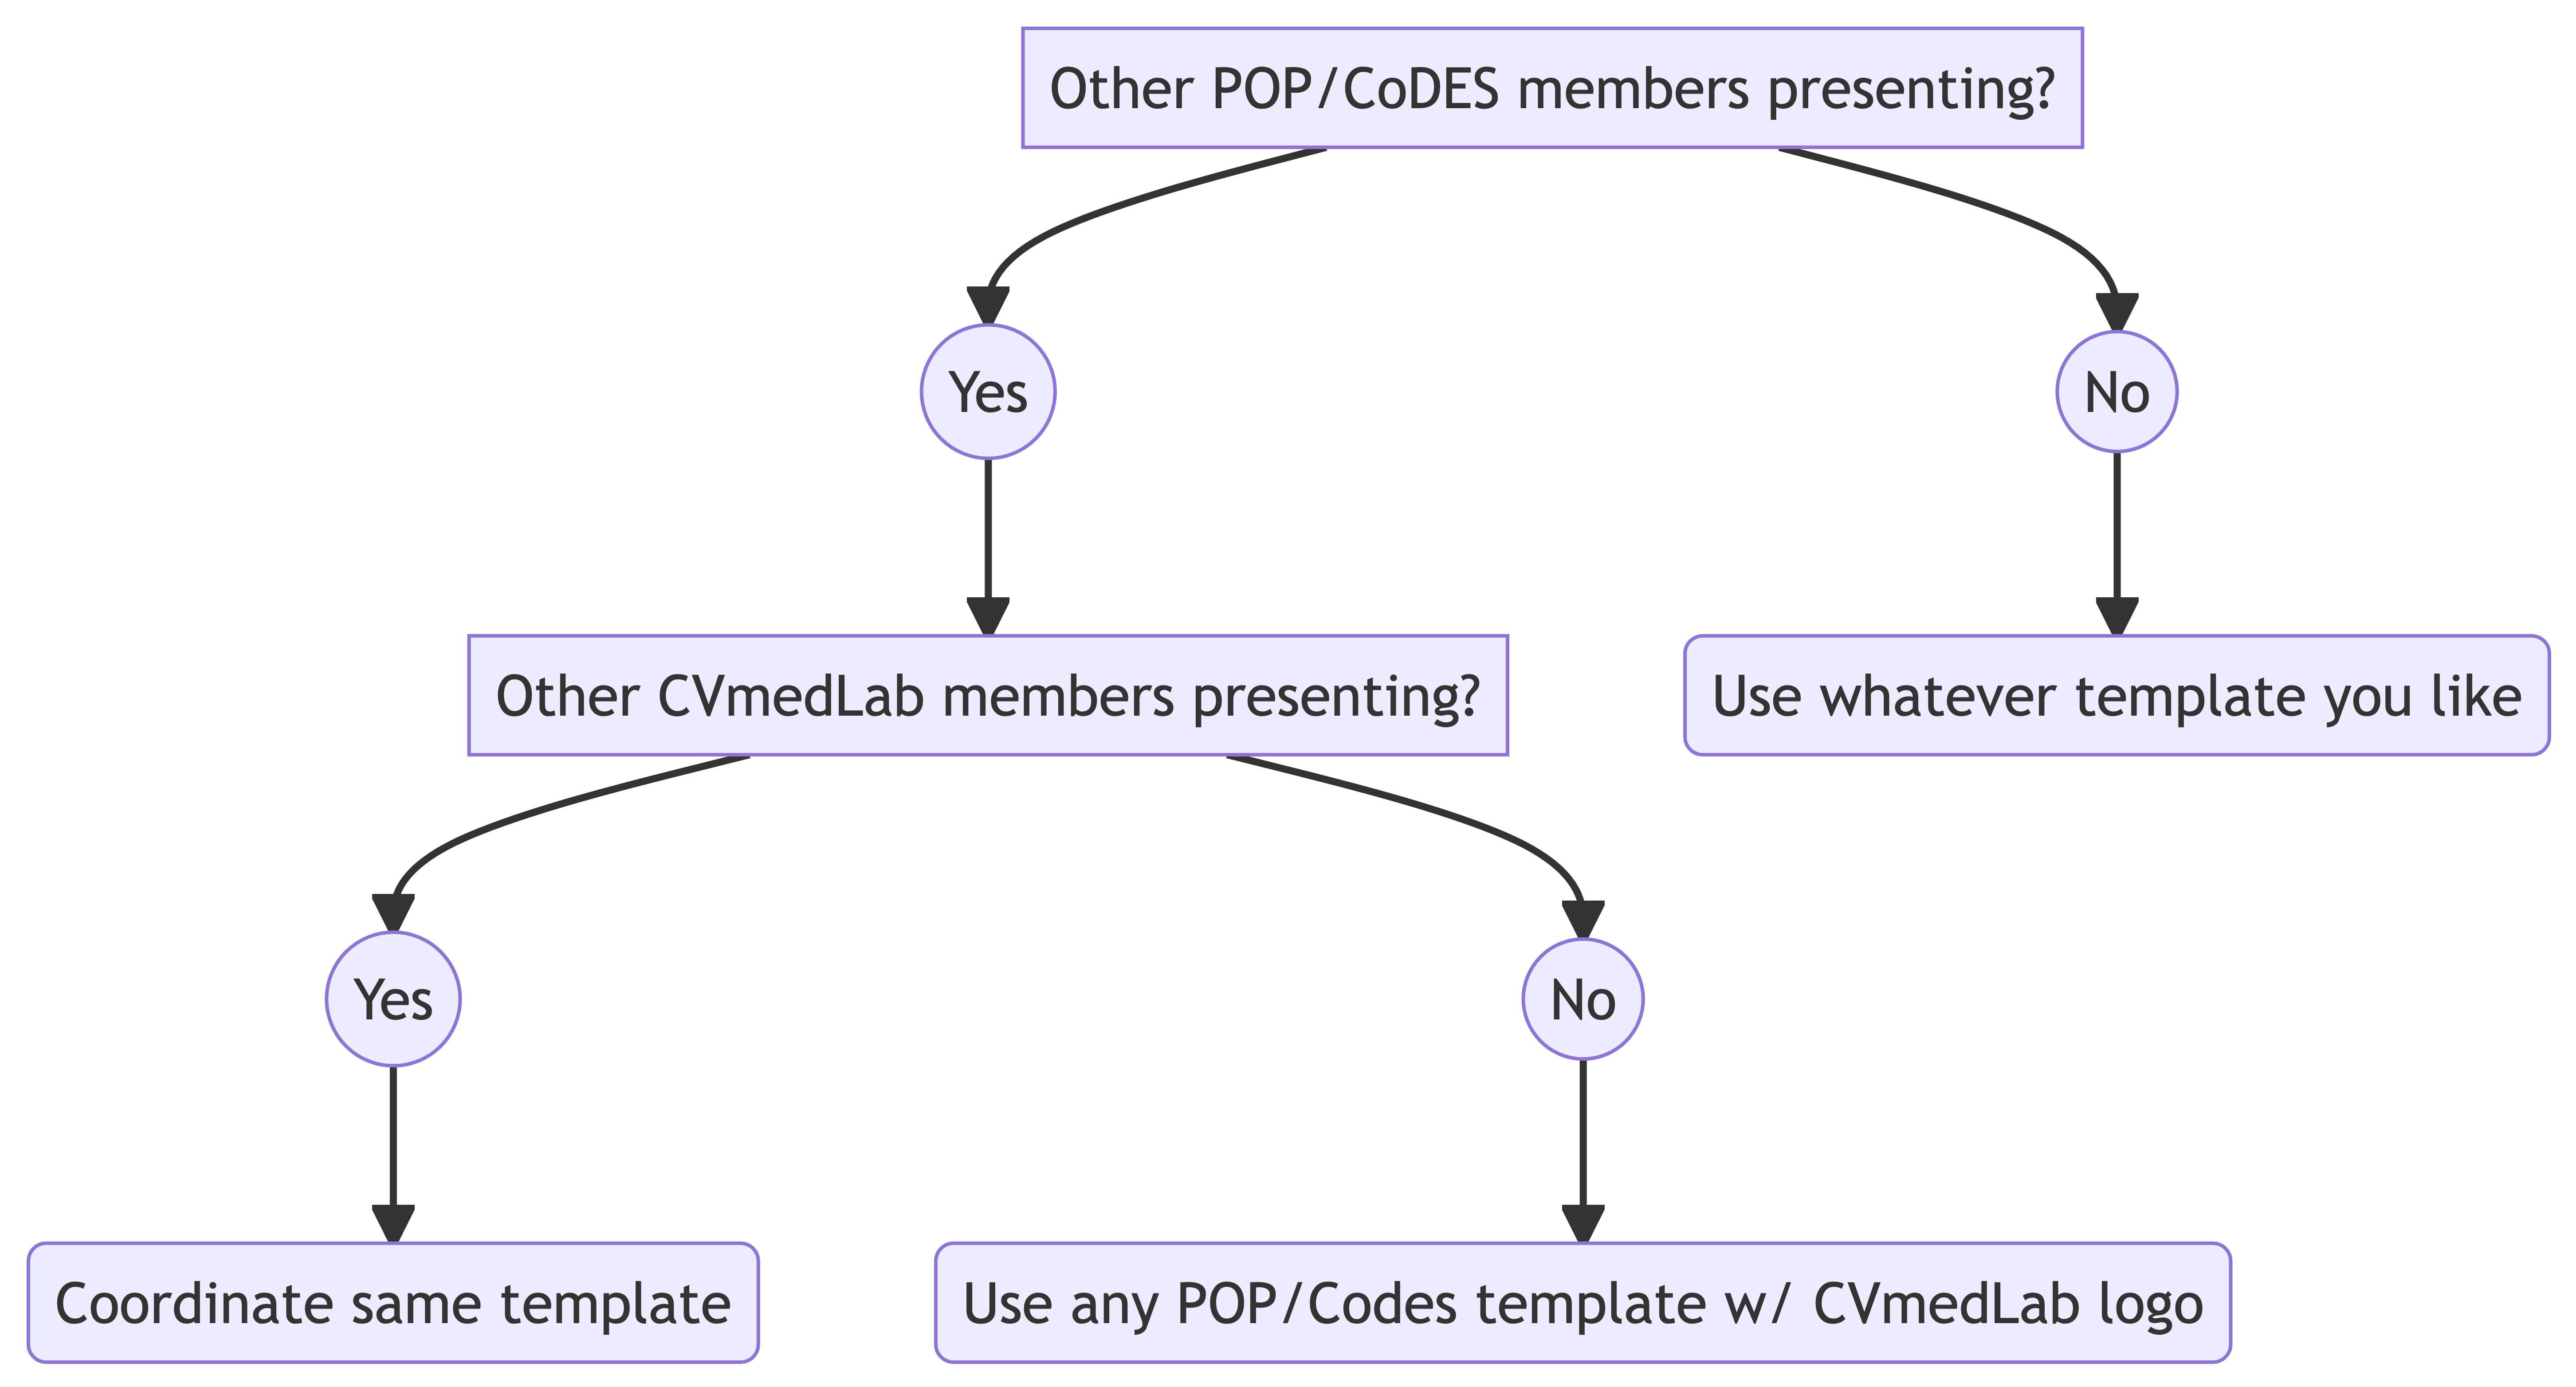
\includegraphics[width=7.57in,height=4.08in]{./conferences_files/figure-latex/mermaid-figure-1.png}

}

\end{figure}

Here are several templates that allow for consistency between lab
presentations, and also with other POP/CoDES presentations:

\begin{figure}

\begin{minipage}[t]{0.50\linewidth}

{\centering 

\raisebox{-\height}{

\href{/assets/templates/posters/poster-template-portrait-2022.pptx}{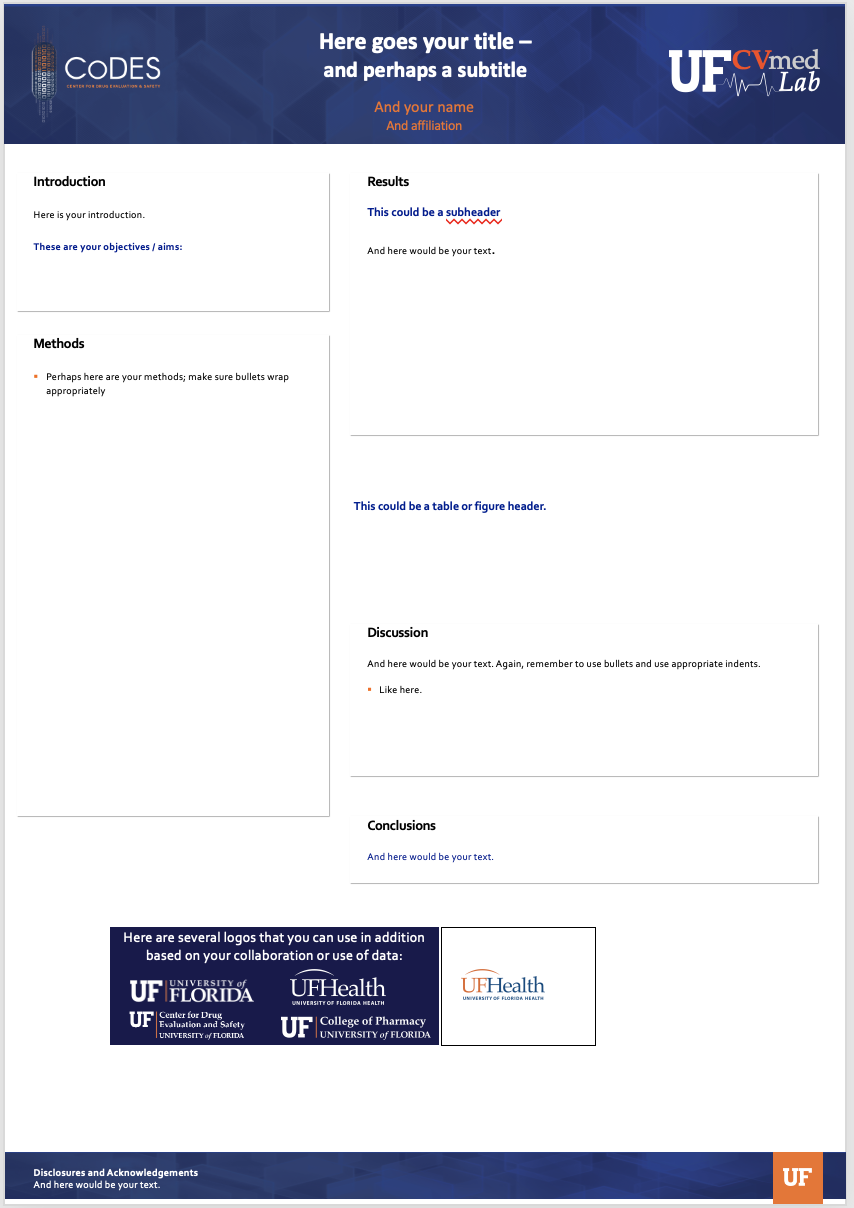
\includegraphics{assets/templates/posters/poster-template-portrait-CoDES.png}}

}

}

\subcaption{\label{fig-anonymous-1}}
\end{minipage}%
%
\begin{minipage}[t]{0.50\linewidth}

{\centering 

\raisebox{-\height}{

\href{/assets/templates/posters/poster-template-portrait-2019-UF.pptx}{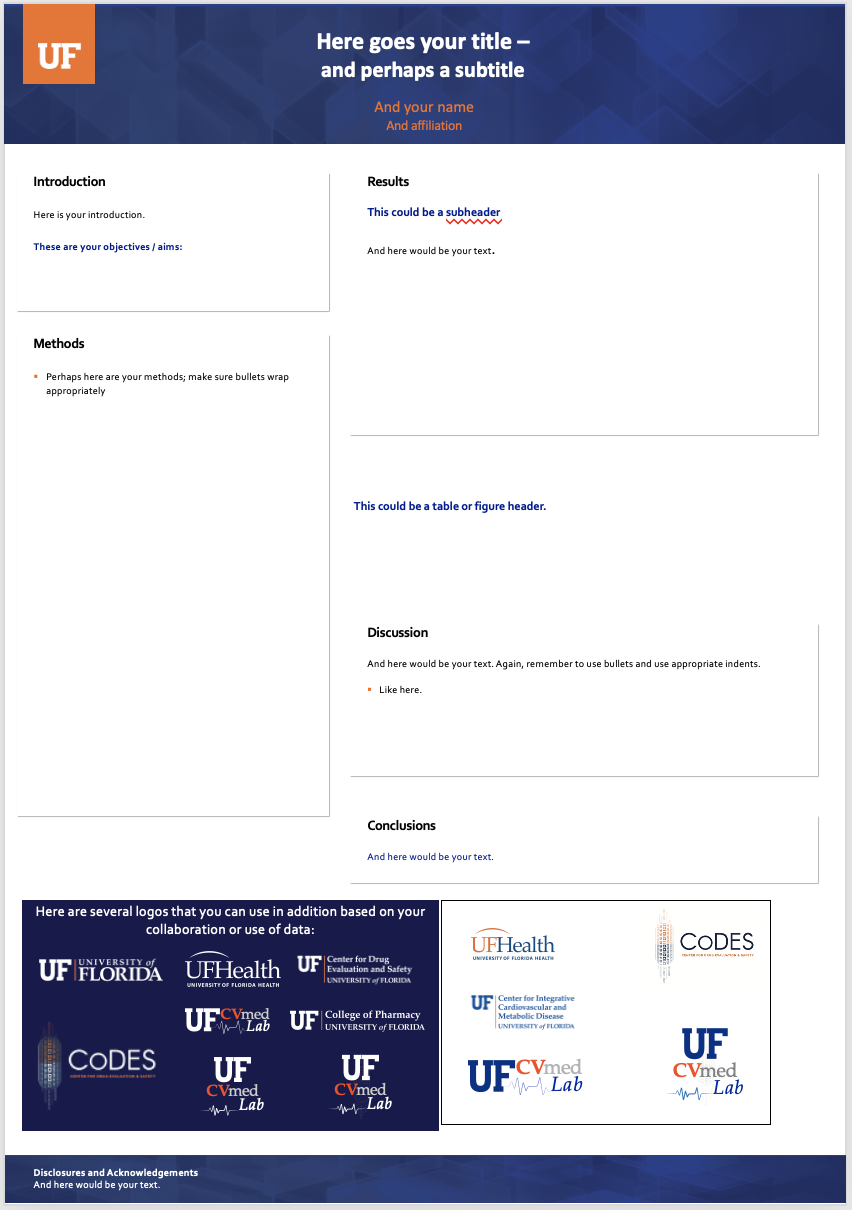
\includegraphics{assets/templates/posters/poster-template-portrait-UF.png}}

}

}

\subcaption{\label{fig-anonymous-2}}
\end{minipage}%

\caption{\label{fig-portrait_posters}Portrait Posters}

\end{figure}

\begin{figure}

\begin{minipage}[t]{0.50\linewidth}

{\centering 

\raisebox{-\height}{

\href{/assets/templates/posters/poster-template-landscape-2022.pptx}{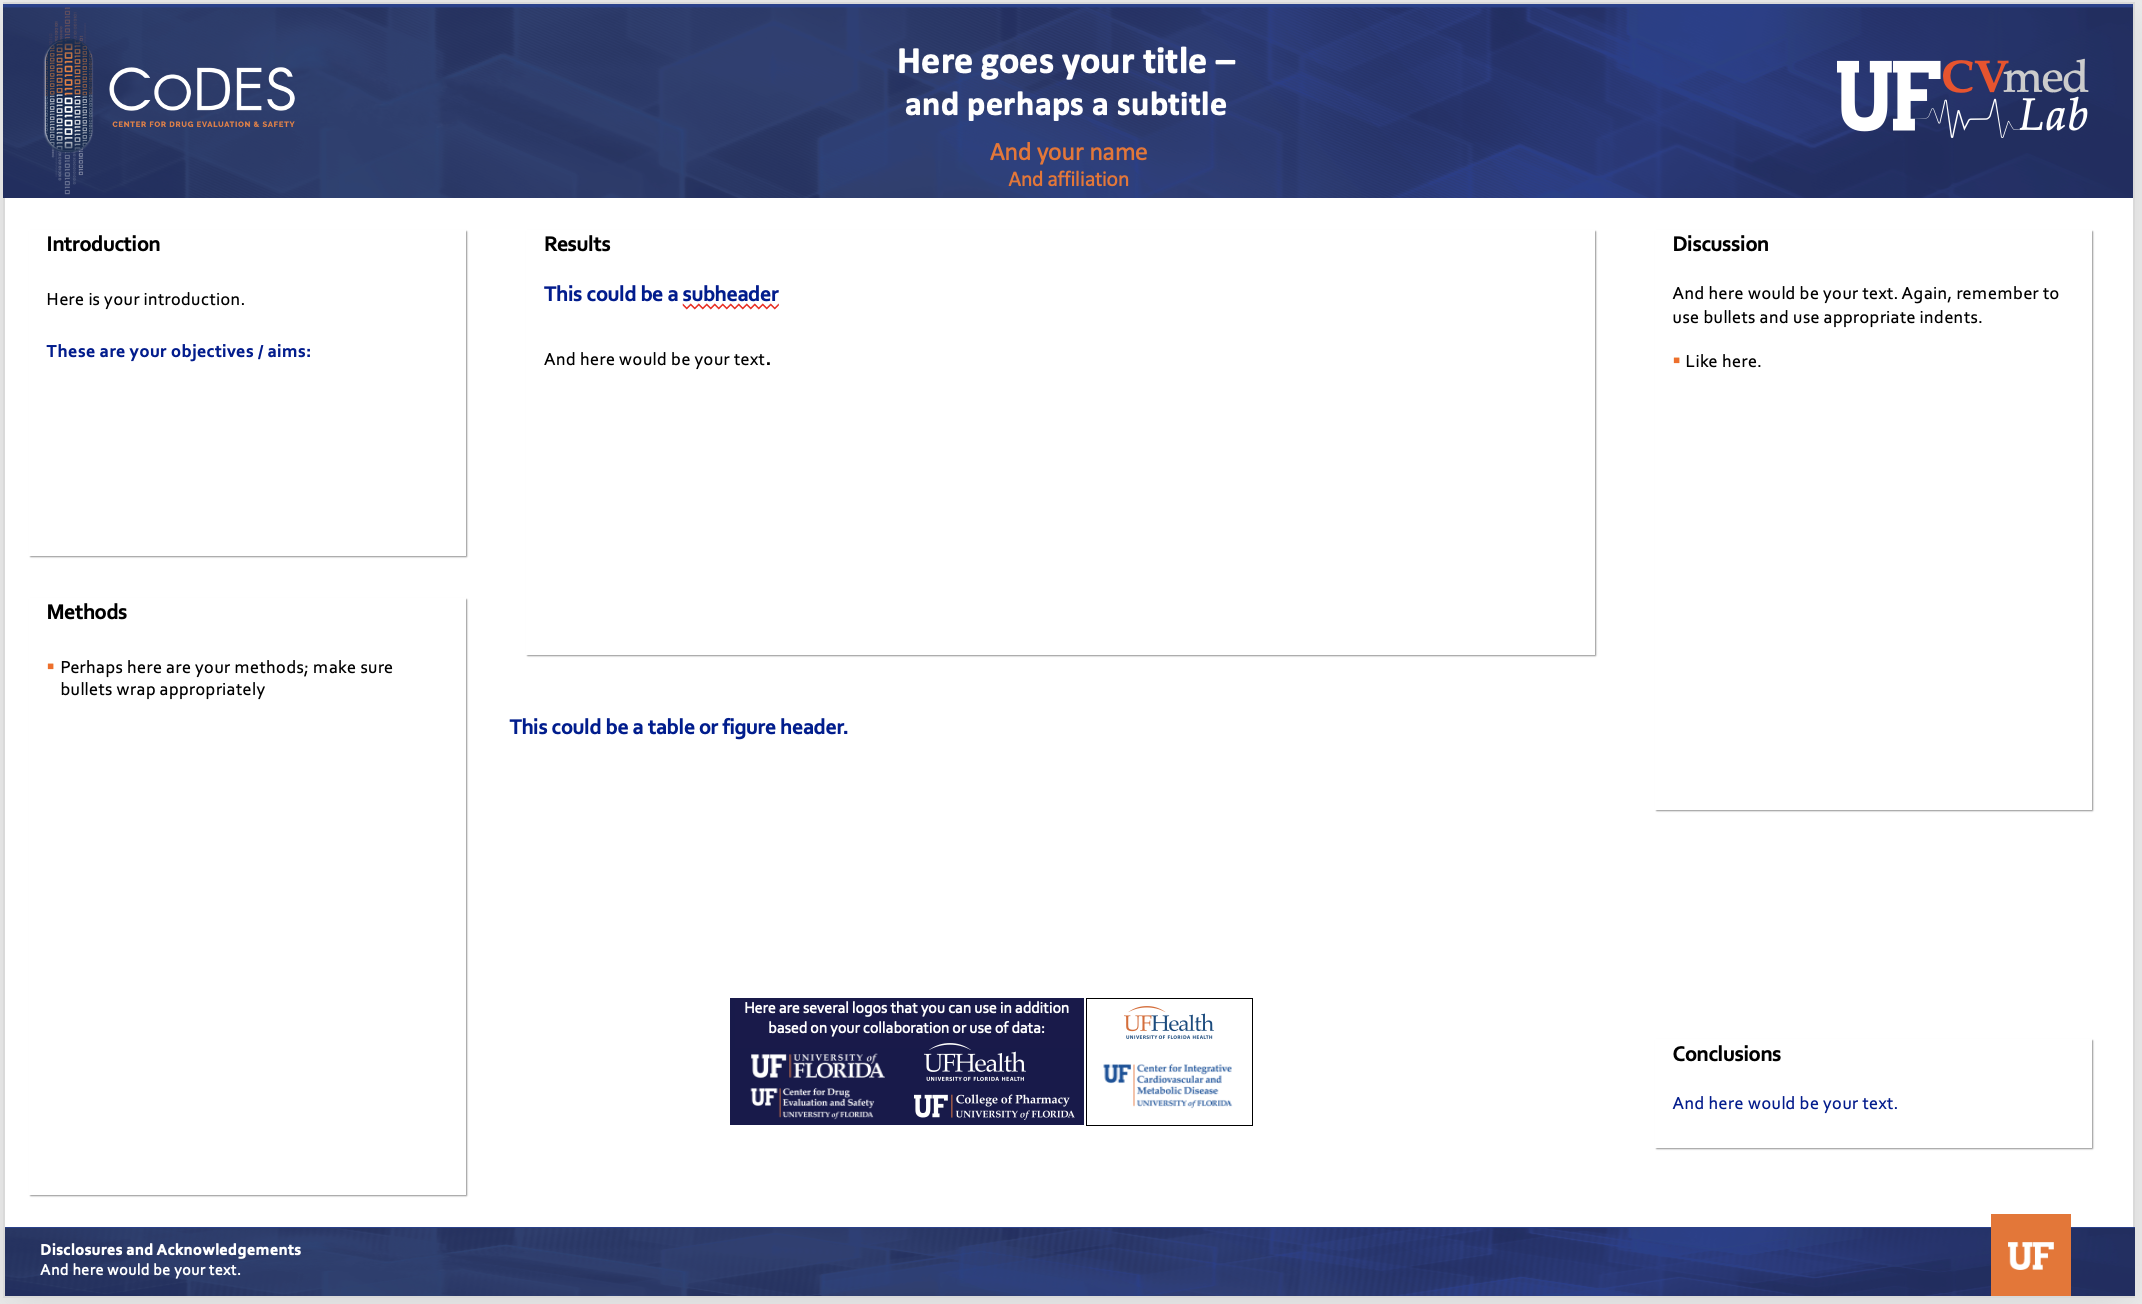
\includegraphics{assets/templates/posters/poster-template-landscape-CoDES.png}}

}

}

\subcaption{\label{fig-anonymous-3}}
\end{minipage}%
%
\begin{minipage}[t]{0.50\linewidth}

{\centering 

\raisebox{-\height}{

\href{/assets/templates/posters/poster-template-landscape-2019-UF.pptx}{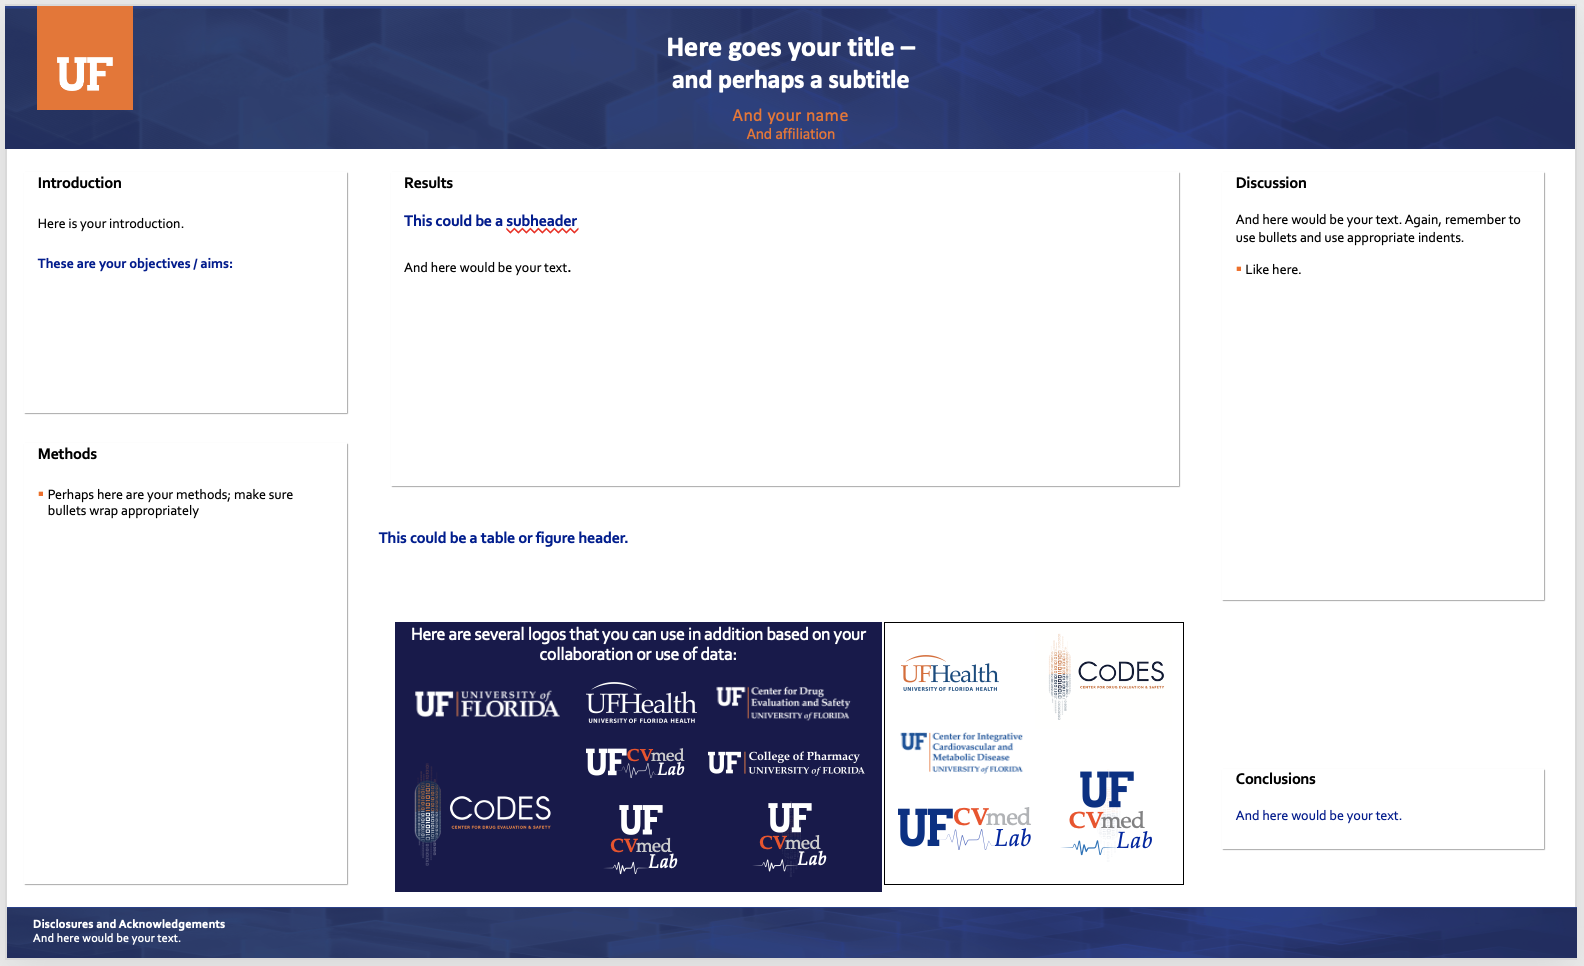
\includegraphics{assets/templates/posters/poster-template-landscape-UF.png}}

}

}

\subcaption{\label{fig-anonymous-4}}
\end{minipage}%

\caption{\label{fig-landscape_posters}Landscape Posters}

\end{figure}

\begin{figure}

\begin{minipage}[t]{0.50\linewidth}

{\centering 

\raisebox{-\height}{

\href{/assets/templates/posters/BP\%20interfering\%20meds\%20poster\%20draft\%20final.pptx}{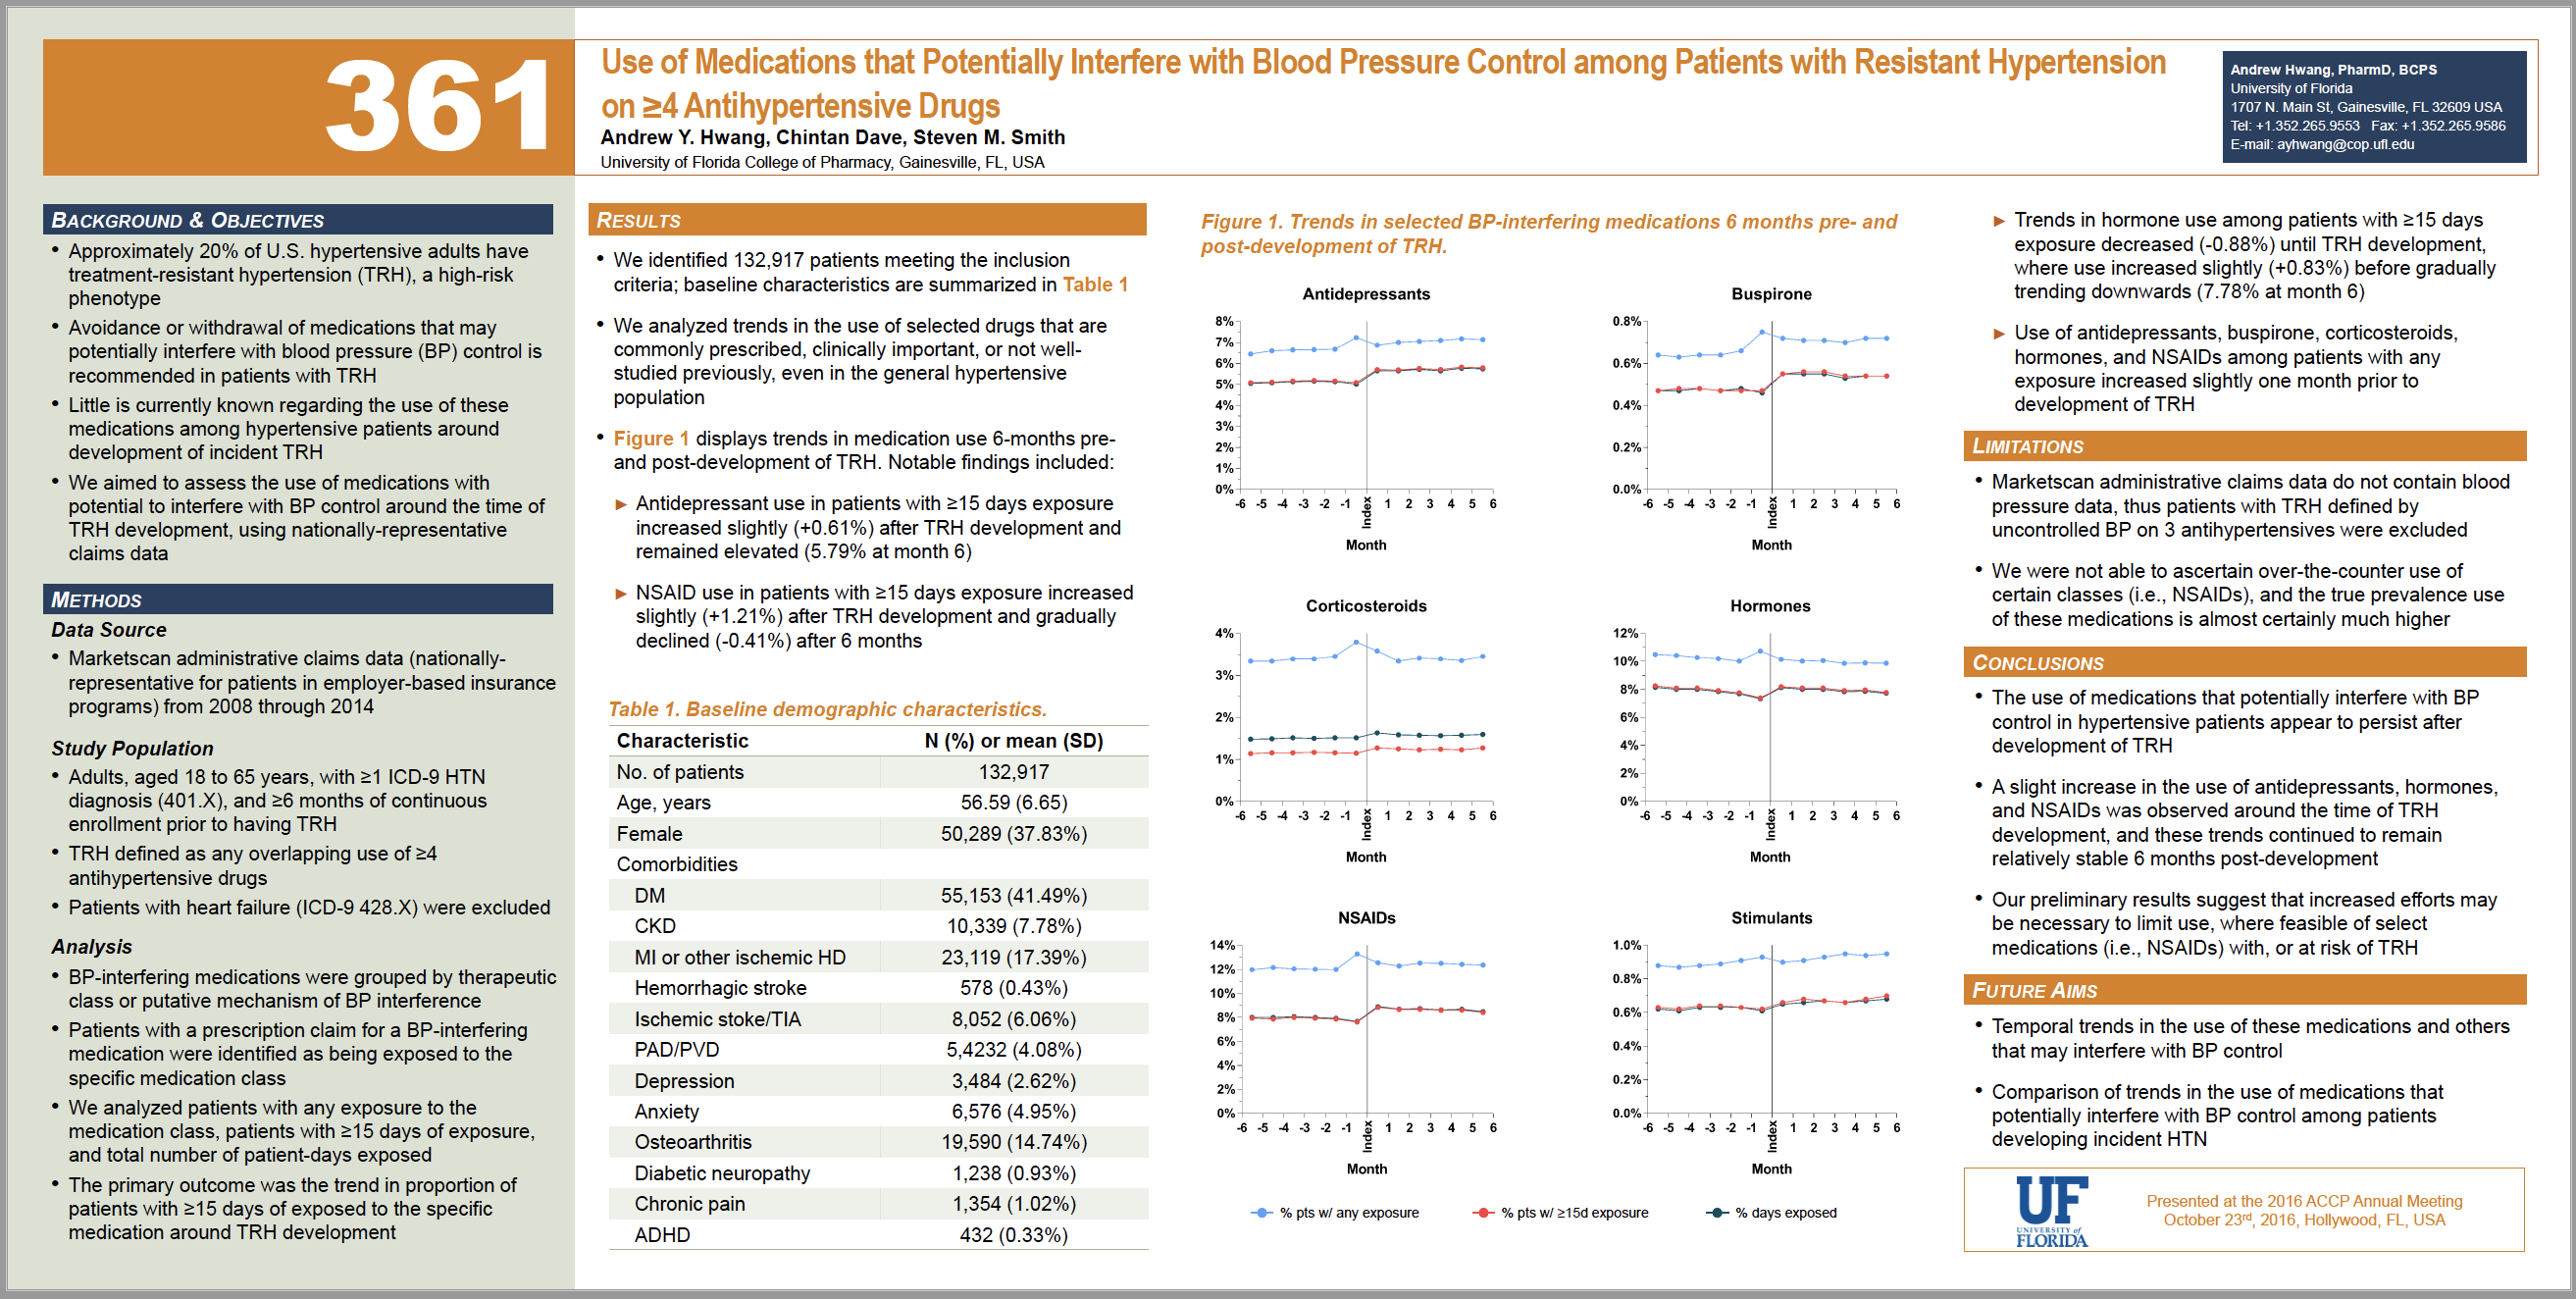
\includegraphics{assets/templates/posters/BP_interfering_meds_poster.png}}

}

}

\subcaption{\label{fig-anonymous-5}}
\end{minipage}%
%
\begin{minipage}[t]{0.50\linewidth}

{\centering 

\raisebox{-\height}{

\href{/assets/templates/posters/ASH\%20Marketscan\%20TRH\%20Trends\%202016\%20FINAL.pptx}{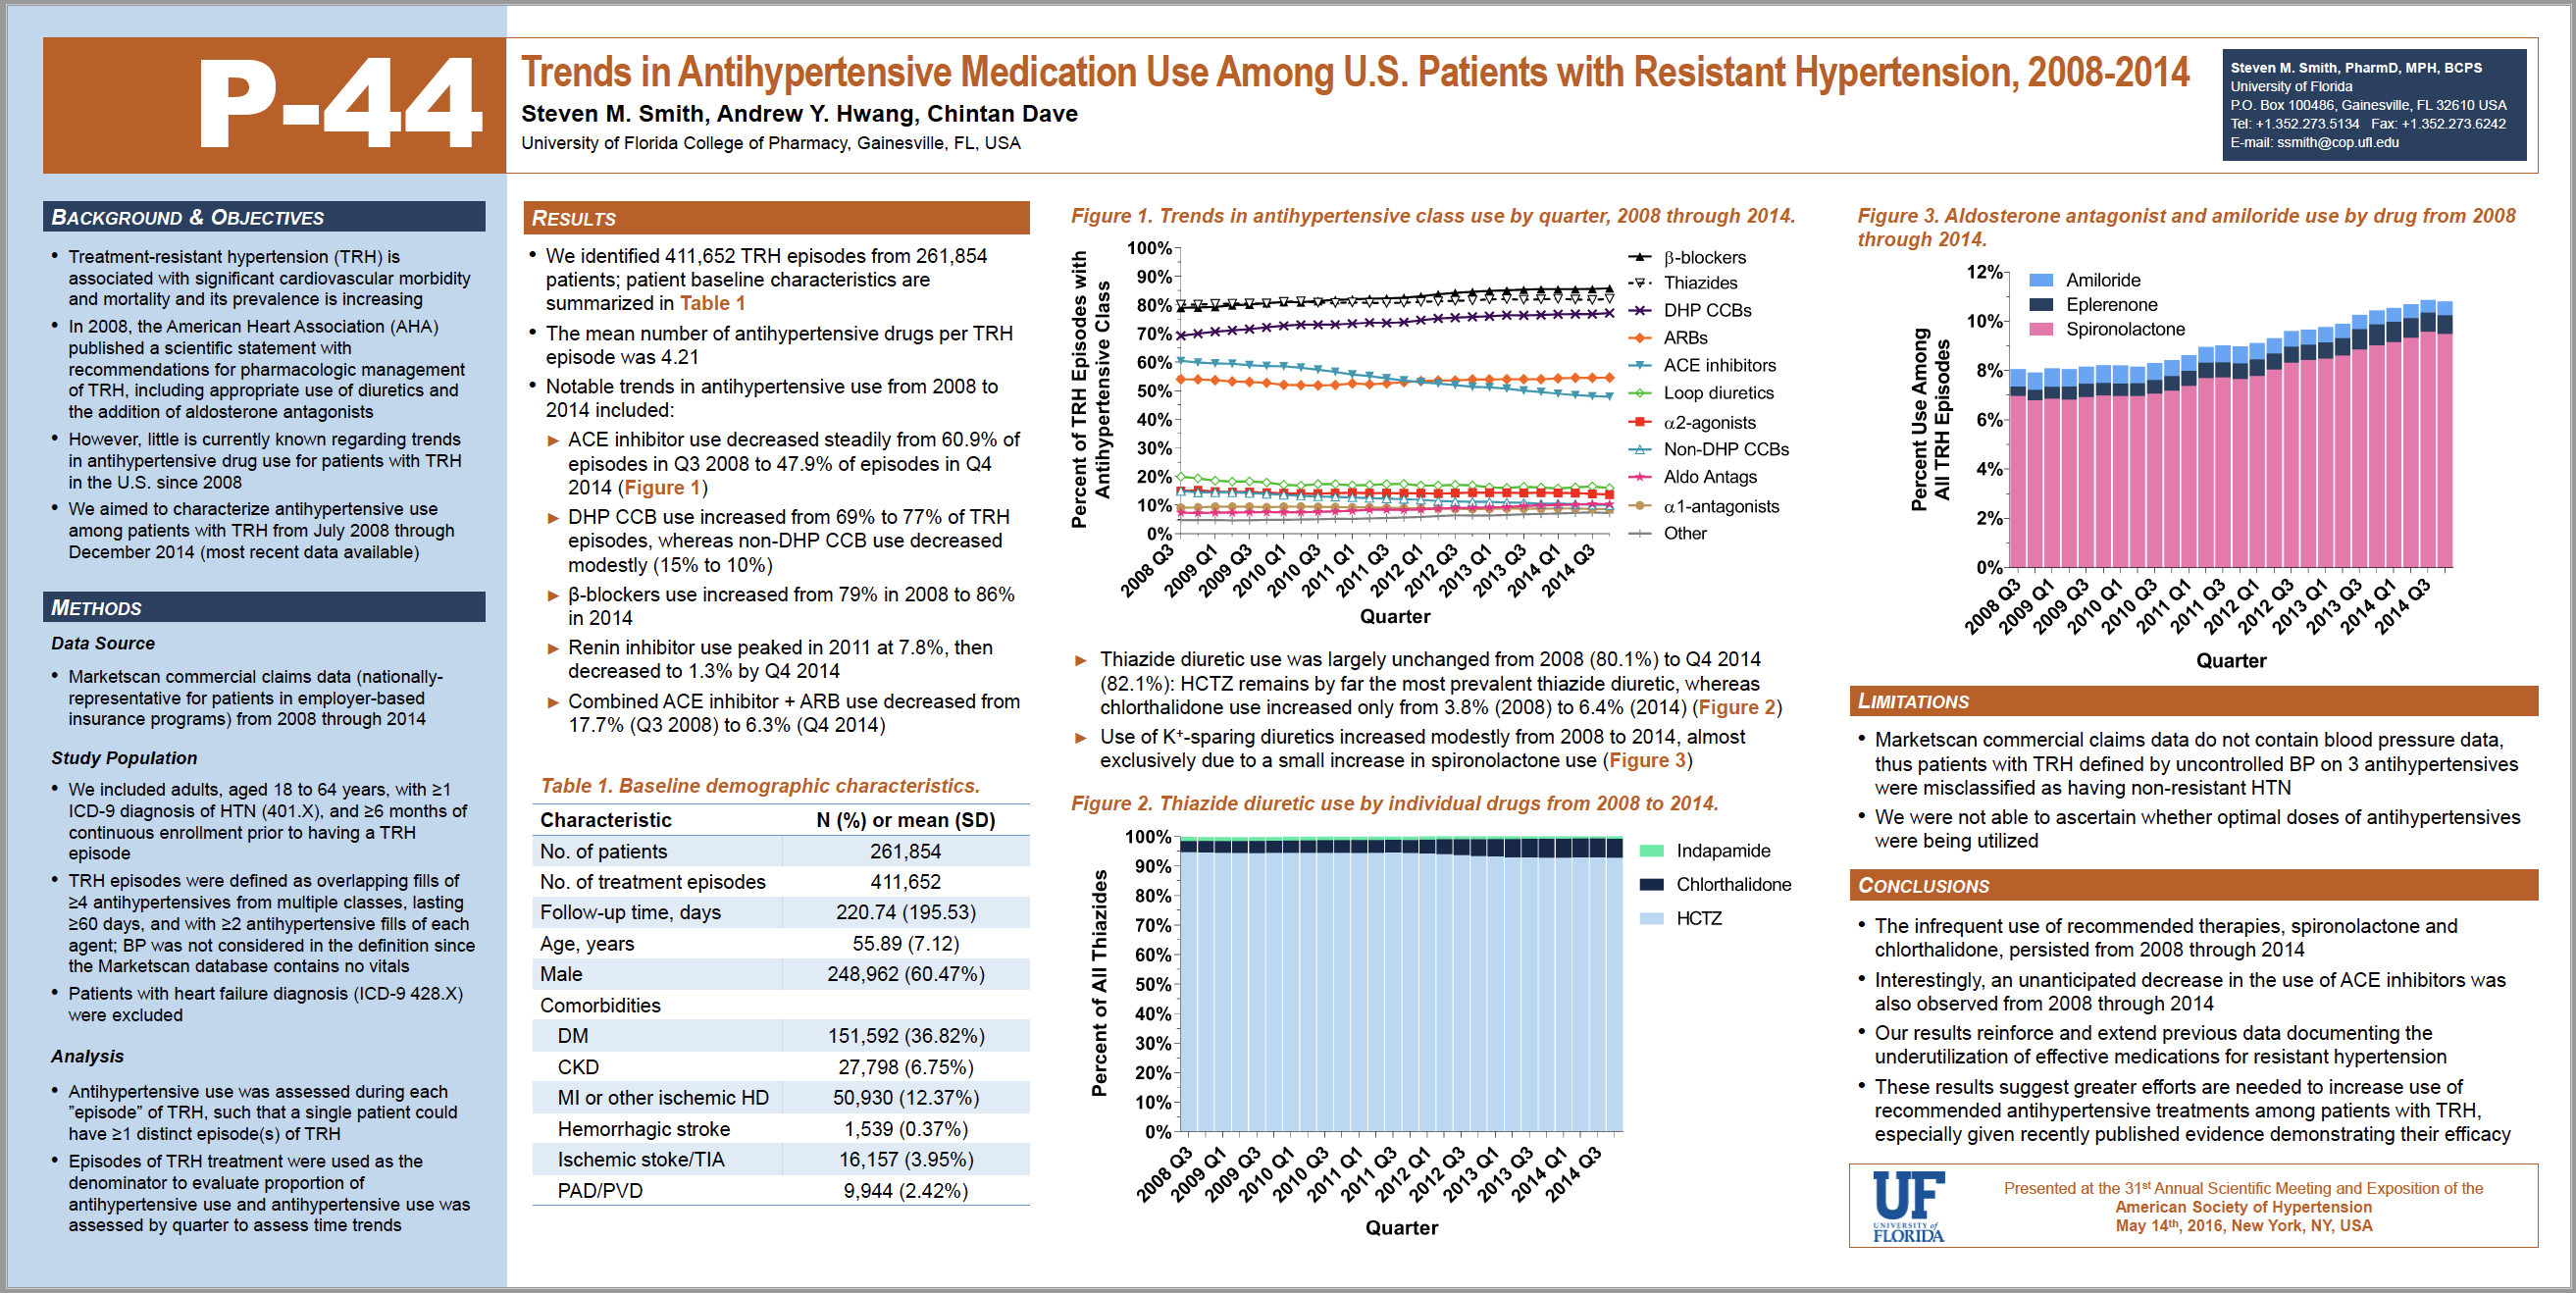
\includegraphics{assets/templates/posters/ASH_TRH_trends_poster.png}}

}

}

\subcaption{\label{fig-anonymous-6}}
\end{minipage}%

\caption{\label{fig-other_posters}Some other templates we've used in the
past}

\end{figure}

\begin{tcolorbox}[enhanced jigsaw, colframe=quarto-callout-note-color-frame, opacityback=0, leftrule=.75mm, bottomrule=.15mm, rightrule=.15mm, left=2mm, toptitle=1mm, colback=white, bottomtitle=1mm, titlerule=0mm, title=\textcolor{quarto-callout-note-color}{\faInfo}\hspace{0.5em}{Note}, arc=.35mm, toprule=.15mm, breakable, coltitle=black, colbacktitle=quarto-callout-note-color!10!white, opacitybacktitle=0.6]

\bookmarksetup{startatroot}

\hypertarget{acknowledging-support}{%
\chapter{Acknowledging Support}\label{acknowledging-support}}

Make sure to consider who supported the work we're presenting. For
example, if \href{https://codes.pharmacy.ufl.edu/}{CoDES} data were
used, or travel support was provided from, e.g.,
\href{https://cicmd.center.ufl.edu/}{CICMD}, or the work was funded in
whole or in part by another organization (e.g., UF
\href{https://pharmacy.ufl.edu/}{COP},
\href{https://www.ctsi.ufl.edu}{CTSI} or an external funder like PhRMA
or AHA), we should make sure these are acknowledged in the poster (or
powerpoint) presentation. If available, consider adding the logo of the
supporter and including appropriate text in the Acknowledgement section
of the poster/presentation.

\end{tcolorbox}

\hypertarget{where-to-print-a-poster}{%
\section{Where to Print a Poster}\label{where-to-print-a-poster}}

UF \href{https://print.at.ufl.edu/help/printing-locations/}{Printing
Services} maintain a list of printing services/locations on UF campus.
For posters, you will need a \textbf{plotter}, which is only available
at some of the locations on the above website.

Additional options can be found at the
\href{https://www.ortho.ufl.edu/poster-service}{Orthopedics and Sports
Medicine Institute}, as well as other businesses in Gainesville (e.g.,
\href{https://target-copy.com/}{Target Copy}), but UF options are likely
to be least expensive.

Your best bet is to \textbf{ask your fellow trainees} where they're
getting their posters printed. New options pop up all the time, and they
can probably give you the best sense of what has worked for them -- and
what hasn't.

\begin{tcolorbox}[enhanced jigsaw, colframe=quarto-callout-tip-color-frame, opacityback=0, leftrule=.75mm, bottomrule=.15mm, rightrule=.15mm, left=2mm, toptitle=1mm, colback=white, bottomtitle=1mm, titlerule=0mm, title=\textcolor{quarto-callout-tip-color}{\faLightbulb}\hspace{0.5em}{Tip}, arc=.35mm, toprule=.15mm, breakable, coltitle=black, colbacktitle=quarto-callout-tip-color!10!white, opacitybacktitle=0.6]

\bookmarksetup{startatroot}

\hypertarget{poster-sizing}{%
\chapter{Poster sizing}\label{poster-sizing}}

Be careful with L x W \emph{dimensions} of your poster file vs.~the
eventual printed poster. The portrait poster templates above are 36''
(W) x \textasciitilde50'' (L) and the landscape poster templates are
\textasciitilde55'' (W) x \textasciitilde35'' (L). Most of the plotter
printers print a maximum of 36'' in one of the dimensions (W or L,
depending on orientation of the poster) and essentially unlimited in the
other dimension. So, both of these will be printed at about 100\% scale.
The other (older) templates are at 18'' x 36'', so would be printed at
200\% scale. The point is, you need to understand at what scale you're
printing -- or better yet, get someone at the printing office to help
scale it correctly.

Finally, your best bet is usually to save your PPTX file to a PDF
(vector-based image) that will print without losing quality at any
adjusted scale. And, where possible, use vector-based figures (SVG, EPS,
or PDF) -- these, too, will scale without losing quality, whereas
raster-based figures (PNG, JPG, TIF, etc..) will not. If you go with the
latter, make sure you save them as big enough images that you don't need
to scale them up substantially to be able to print a large poster.

\end{tcolorbox}

\hypertarget{presentation-templates}{%
\section{Presentation Templates}\label{presentation-templates}}

So you got your abstract accepted as a platform presentation - congrats!
We have templates for these too. However, check closely the invitation
from the meeting organizers. Often platform presentations are expected
to use a template from the meeting, which provides consistency across
presentations at the meeting.

Presentation Templates:

\begin{itemize}
\item
  \href{/assets/templates/presentations/2017-cop-16x9-external-presentations-1.pptx}{COP
  Template 1} - basic template
\item
  \href{/assets/templates/presentations/2017-cop-16x9-external-presentations-2.pptx}{COP
  Template 2} - basic template
\item
  \href{/assets/templates/presentations/UF-PowerPoint_Template_2022.potx}{UF
  Template 2022} - this has a ton of ideas for different types of slides
  worth a look even if just for ideas)
\item
  \href{/assets/templates/presentations/UF_branded_PowerPoint_template_widescreen.ppt}{Older
  UF Template}
\end{itemize}

The \href{https://brandcenter.ufl.edu/downloads/}{UF Brand Center} also
has a lot of other assets that can be added to presentations or posters
and is worth looking through.

\hypertarget{support-for-presenting-at-conferences}{%
\section{Support for Presenting at
Conferences}\label{support-for-presenting-at-conferences}}

The lab will cover the cost of poster printing for posters of lab
research. Discuss with the POP Administrative Assistant (Katherine or
other) how best to pay for or get reimbursed for this.

You should seek out sources of support for travel and other costs
associated with attending conferences. The
\href{https://cicmd.center.ufl.edu/}{CICMD} helps offset travel if you
have an accepted poster/presentation (you will need to acknowledge the
support of CICMD). Many conferences also offer travel support for
trainees.

Speak to your colleagues in the department for other possible sources of
support

\bookmarksetup{startatroot}

\hypertarget{sec-papers}{%
\chapter{Papers}\label{sec-papers}}

Hopefully this is not coming as a surprise, but you will write a lot of
papers (manuscripts). It's helpful to have a semi-standard way of
putting these together.

\begin{tcolorbox}[enhanced jigsaw, colframe=quarto-callout-note-color-frame, opacityback=0, leftrule=.75mm, bottomrule=.15mm, rightrule=.15mm, left=2mm, toptitle=1mm, colback=white, bottomtitle=1mm, titlerule=0mm, title=\textcolor{quarto-callout-note-color}{\faInfo}\hspace{0.5em}{Note}, arc=.35mm, toprule=.15mm, breakable, coltitle=black, colbacktitle=quarto-callout-note-color!10!white, opacitybacktitle=0.6]

Although journals sometimes vary in their specific requirements for a
submitted manuscript, there is a growing movement in scientific
publishing to allow researchers to submit manuscripts with only very
basic formatting requirements on the first submission, and if the
journal is interested, they will then require more specific formatting
requirements on any revisions requested. This is good news for us, as it
reduces how much re-formatting we need to do if a manuscript does not
get traction at a few journals.

\end{tcolorbox}

\hypertarget{general-principles}{%
\section{General Principles}\label{general-principles}}

Some general principles for drafting your manuscript:

\begin{itemize}
\item
  If you haven't already, check out the CVmedLab lab doc called
  \href{https://cvmedlab.org/labdocs/writing.html}{Scientific Writing}
\item
  Each major section of a manuscript should begin on a new page: title
  page, abstract, introduction, methods, results, discussion,
  references, tables (each on a new page), and figures (each on a new
  page).
\item
  Everything should be Arial font, size 11; every page (except title
  page) should be double-spaced; title page should be single-spaced
\item
  Major headings (Introduction, Methods, etc..) should be \textbf{bold}.
  Second-level headings should be \emph{italic}. Third-level headings
  should be underlined.
\item
  Pages should be numbered (preferably top right corner).
\item
  Figures trump tables in terms of presenting all but the simplest data.
  Figures are much more likely to be re-used by others in presentations,
  review articles, news articles, etc\ldots{}
\item
  Tables come before figures sequentially in the manuscript.
\item
  Figures should be vector images (.SVG preferably; alternatively,
  .EPS); these do not lose quality when scaled up (zoomed in on). Both
  \href{https://documentation.sas.com/doc/en/pgmsascdc/9.4_3.5/lrcon/n0ezld96mjxs08n1lvoj5mtb4opl.htm}{SAS}
  and \href{https://ggplot2.tidyverse.org/reference/ggsave.html}{R} can
  output SVG files fairly easily. If you're designing figures (as
  opposed to outputting data-based plots), consider
  \href{https://info.apps.ufl.edu/adobeatufapps/}{Adobe Illustrator}
  (smallish annual fee) or \href{https://app.diagrams.net/}{draw.io}
  which is good for creating diagrams (design schematics, flow charts,
  etc..) and can output SVG files.
\item
  Regardless of what the journal says, embed figure(s) directly in the
  manuscript file; if the journal requests that figures be submitted
  separately, do that also (in addition to embedding them), but keep
  them embedded either way. This makes it easier for reviewers to see
  figures at the size you want them to, rather than what the journal's
  submission software includes them in the PDF as.
\item
  Most journals allow for unlimited tables/figures in the Supplement.
  You should consider using a supplement liberally, meaning putting
  tables/supplements in the figure if you think they'll be of interest
  to only a limited section of the readership of a journal. Most often,
  we will include study design figures and patient flow diagrams in
  these, as well as, e.g., sensitivity analysis results. They also can
  be used for additional methodologic details if you find the main text
  Methods section becoming too bloated. Basically, anything potentially
  of interest to at least some readers (or that can be helpful in
  mitigating likely reviewer critiques) should go in the Supplement.
\item
  Everything in the Supplement can be single-space; if the Supplement is
  particularly long, consider adding a Table of Contents page (page
  after the title page)
\end{itemize}

\hypertarget{references-1}{%
\section{References}\label{references-1}}

You should familiarize yourself with reference management software,
which will make your life immensely easier when writing manuscripts.
Dr.~Smith prefers \href{https://www.mendeley.com/}{Mendeley} or
\href{https://www.zotero.org/}{Zotero}, both of which are free.
\href{https://www.myendnoteweb.com/}{EndNote web} is also acceptable.
The important point is to pick one that works for you. Don't manually
edit/re-order references; this will be a waste of your time.

\hypertarget{manuscript-templates}{%
\section{Manuscript Templates}\label{manuscript-templates}}

\hypertarget{word-doc-template}{%
\subsection{Word Doc template}\label{word-doc-template}}

The most common format we work with will be a Word document. Here's a
\href{/assets/templates/papers/word_paper_template.dotx}{template} you
can use to get started on a manuscript. And, here is a
\href{/assets/templates/papers/word_supplement_template.dotx}{template
for a supplement}. To use, in Word, do File -\textgreater{} New from
Template\ldots{} -\textgreater{} Select the saved template file from the
above links -\textgreater{} get to editing.

\hypertarget{quarto-doc}{%
\subsection{Quarto Doc}\label{quarto-doc}}

To do\ldots{}

\hypertarget{support}{%
\section{Support}\label{support}}

The \href{https://cicmd.center.ufl.edu/}{CICMD} offers support for
offsetting costs of manuscripts (open access or page fees). Discuss with
Dr.~Smith whether you should submit a request for funding.

\bookmarksetup{startatroot}

\hypertarget{sec-computing}{%
\chapter{Computing}\label{sec-computing}}

To do.

\bookmarksetup{startatroot}

\hypertarget{sec-data}{%
\chapter{Data Resources}\label{sec-data}}

\href{https://pop.pharmacy.ufl.edu/}{POP}/\href{https://codes.pharmacy.ufl.edu/}{CoDES}
have a wealth of data resources that are generally refreshed/updated
every 1-2 years, and available to the graduate program, including you.
Our lab uses primarily OneFlorida+ data (which includes FL Medicaid),
Marketscan, and Medicare. Read on below for info on each. You can access
to any/all of the above for your own independent research projects or
thesis work, though some have fees attached which you'll need to discuss
with Dr.~Smith.

Most of these data are housed on ResVault virtual machines or the POP
high-performance server. See Chapter~\ref{sec-computing} for more
information.

\hypertarget{electronic-health-record-ehr-data}{%
\section{Electronic Health Record (EHR)
data}\label{electronic-health-record-ehr-data}}

\hypertarget{oneflorida}{%
\subsection{OneFlorida+}\label{oneflorida}}

\href{https://onefloridaconsortium.org/}{OneFlorida+} is one of 11
clinical research networks (CRNs) that comprise the
\href{https://www.pcornet.org/}{Patient-Centered Ourcomes Research
network (PCORnet)}. Quite a bit of our work is done on OneFlorida+ data,
or data from OneFlorida+ and other PCORnet CRNs. The good news is they
all adhere to the \href{https://pcornet.org/data/}{PCORnet common data
model} (scroll to the bottom of the page), which you will need to
familiarize yourself with if you're working on OneFl+/PCORnet data. In
particular, you'll need to familiarize yourself with the relevant
\href{https://pcornet.org/wp-content/uploads/2022/01/PCORnet-Common-Data-Model-v60-2020_10_221.pdf}{tables
and variables}. If you're unsure whether you'll be working with
OneFl+/PCORnet data, ask Dr.~Smith.

OneFlorida+ includes EHR data from health system partners across Florida
(UF, University of Miami, University of South Florida, Orlando Health,
Florida Hospital {[}Orlando{]}, Tallahassee Memorial, and others), as
well as University of Alabama-Birmingham (UAB) and Emory University. In
addition, it contains Florida Medicaid claims data. Data are generally
available from \textasciitilde2012 onward. As you'll see on reviewing
the common data model, the available data are generally structured data
(rather than unstructured clinical texts like provider notes, imaging
reports, etc..).

\hypertarget{ufhealth-data}{%
\subsection{UFHealth data}\label{ufhealth-data}}

The \href{https://idr.ufhealth.org/}{UF integrated data repository} is a
database of UFHealth EHR data, including both structured and
unstructured data. The IDR has an i2b2 implementation which can be used
for simple queries, i.e., to find counts of patients that meet certain
criteria. The IDR i2b2 implementation can be found
\href{https://i2b2.idr.ufhealth.org/}{here} (you'll need to register for
an account
\href{https://idr.ufhealth.org/research-services/feasibility-cohort-discovery/}{here}
and you'll need to be on campus or on the HSC VPN to access i2b2).

We are currently in the process of linking UFHealth data with our
Medicare claims data for patients in both data sources.

\hypertarget{claims-data}{%
\section{Claims data}\label{claims-data}}

Major claims data sources housed in POP/CoDES include CMS data and IBM
Marketscan. Brief descriptions are below. Additional information can be
found
\href{https://codes.pharmacy.ufl.edu/resources/data-sources/}{here}.

\hypertarget{cms-data-medicare-medicaid}{%
\subsection{CMS data (Medicare,
Medicaid)}\label{cms-data-medicare-medicaid}}

\hypertarget{medicaid}{%
\subsubsection{Medicaid}\label{medicaid}}

Medicaid Analytic eXtract (MAX) and T-MSIS Analytic Files (TAF) data
contain claims for medical care and drug benefits received by
beneficiaries with Medicaid insurance coverage, the state-run programs
for low-income and categorically eligible individuals and families.
CoDES has in-house MAX data for over \textgreater120 million
beneficiaries residing in the 29 most populous states from 1999-2010
(AL, AR, CA, FL, GA, IA, ID, IL, IN, KS, KY, LA, MA, MN, MO, MS, NC, NE,
NJ, NM, NY, OH, SC, TN, TX, VA, WA, WI, WV) and national data (all 50
states plus the district of Columbia) from 2011-2016.

Medicaid data has been linked to birth certificates from the Florida
Department of Health (1999-2014), Texas Department of State Health
Services (1999-2012) and New Jersey Department of Health (1999-2010).
The entire national Medicaid data set includes validated mother-infant
linkages.

\hypertarget{medicare}{%
\subsubsection{Medicare}\label{medicare}}

Medicare data include claims for inpatient, skilled care nursing
facility, and hospice care (Part A) as well as outpatient care (Part B)
and prescription drugs (Part D). CoDES center has a somewhat complicated
sample of Medicare, due in part to our desire to link UFHealth EHR data
with Medicare data.

Basically, the current sample includes the following:

\begin{itemize}
\tightlist
\item
  A 5\% national Medicare sample (random sample of 5\% of Medicare
  patients nationwide who meet the above criteria for parts A, B, and D)
  for the years 2011 through 2015 plus 1 million beneficiaries in FL
  sampled from individuals who reside in the UF Health catchment area
  (to ensure we could link most UFHealth patients)
\item
  A 15\% national Medicare beneficiaries plus the entire state of
  Florida for 2016-2018, totaling \textgreater8 million lives.
\end{itemize}

We are anticipating continuing to grow the data (additional years).

ResDAC contains excellent
\href{https://resdac.org/file-availability}{documentation of the
Medicare files}, variables, and availability from year-to-year. If
you're going to use Medicare data, you'll need to get to know these data
dictionaries.

\hypertarget{marketscan}{%
\subsection{Marketscan}\label{marketscan}}

The IBM Marketscan Commericial claims database includes 2005-2020 health
insurance claims for inpatient, outpatient, and outpatient pharmacy
encounters, as well as enrollment data from large employers and health
plans across the United States who provide healthcare coverage for their
employees, their spouses, and dependents. The current dataset includes
\textgreater192 million lives.

The Medicare Supplemental data includes 2005-2020 enrollment records
along with inpatient, outpatient, ancillary, and drug claims for
\textgreater12.9 million retirees in the United States with Medicare
supplemental coverage through privately-insured fee-for-service,
point-of-service, or capitated health plans.

The Health Risk Assessment (HRA) data includes 2012-2018 self-reported
biometric and health-related behavioral data obtained through surveys of
employees of large US corporations and health plans. HRA is linked to
medical, pharmacy, and enrollment data for these employees in the
Commercial claims data (above) and used to examine the relationships
between health behaviors/risk and health outcomes or medical
expenditures. Linked data is available for about 5\% of beneficiaries.

\hypertarget{others}{%
\section{Others}\label{others}}

There's much too much to make this a comprehensive list, but here are
some additional data resources that are either publicly-available or
available to us by virtue of collaborations within UF, and may be of
interest to you/the lab for some of our work.

\hypertarget{clinical-trialprospective-cohort-data}{%
\subsection{Clinical trial/prospective cohort
data}\label{clinical-trialprospective-cohort-data}}

\begin{itemize}
\item
  \href{https://biolincc.nhlbi.nih.gov/home/}{NHLBI BioLINCC} -
  NHLBI-funded clinical trial and prospective cohort data

  \begin{tcolorbox}[enhanced jigsaw, colframe=quarto-callout-note-color-frame, opacityback=0, leftrule=.75mm, bottomrule=.15mm, rightrule=.15mm, left=2mm, toptitle=1mm, colback=white, bottomtitle=1mm, titlerule=0mm, title=\textcolor{quarto-callout-note-color}{\faInfo}\hspace{0.5em}{Note}, arc=.35mm, toprule=.15mm, breakable, coltitle=black, colbacktitle=quarto-callout-note-color!10!white, opacitybacktitle=0.6]

  We currently have access to
  \href{https://www.nejm.org/doi/full/10.1056/nejmoa1511939}{SPRINT} and
  \href{https://www.nejm.org/doi/full/10.1056/nejmoa1001286}{ACCORD}
  trial data - ask Dr.~Smith if interested being added to the DUA for
  these trials

  \end{tcolorbox}
\item
  \href{https://jamanetwork.com/journals/jama/fullarticle/197761}{INVEST
  trial} - we have access to the INVEST trial data, which was a large
  international trial (22.5k individuals enrolled) comparing a calcium
  channel blocker vs.~beta-blocker treatment strategy in patients aged
  ≥50 years with hypertension + coronary artery disease. Includes
  adjudicated cardivoascular events, as well as all-cause death data
  through at least 2015.
\item
  \href{https://www.sciencedirect.com/science/article/pii/S0735109799000820?via\%3Dihub}{WISE
  cohort} - we have access to the Women's Ischemia Syndrome Evaluation
  (WISE) cohort, which was a multisite prospective cohort study of women
  with suspected myocardial ischemia.
\item
  \href{https://jamanetwork.com/journals/jamainternalmedicine/fullarticle/414930}{Women
  Take Heart} - we have access to the Women Take Heart cohort, which was
  a Chicago-based prospective cohort study of \textasciitilde8k women
  without cardiovascular disease, enrolled in 1992 and with death
  follow-up through at least 2008.
\item
  \href{https://www.sciencedirect.com/science/article/abs/pii/S0002870321000776?via\%3Dihub}{WARRIOR
  trial} - The Women's IschemiA TRial to Reduce Events In
  Non-ObstRuctive CAD is a multicenter, prospective, randomized, blinded
  outcome evaluation (PROBE design) of a pragmatic strategy of intensive
  medical therapy (incl.~ACEI or ARB + statin) vs usual care in 4,422
  symptomatic women with ischemia and no obstructive coronary artery
  disease (INOCA)
\end{itemize}

\hypertarget{publicly-available-datasets}{%
\subsection{Publicly-Available
datasets}\label{publicly-available-datasets}}

The CDC curates a number of valuable datasets that are relatively easy
to access and generally offer cleaned, curated datasets that are
analysis-ready. Some common ones we use/see in our field include:

\begin{itemize}
\item
  \href{https://www.cdc.gov/nchs/nhanes/index.htm}{National Health and
  Nutrition Examination Survey (NHANES)} - a complex survey design that
  is completed every 2 years and allows for inference about what is
  happening across the non-instutitionalized U.S. population
\item
  \href{https://www.cdc.gov/nchs/ahcd/index.htm}{National Ambulatory
  Medical Care Survey (NAMCS)} - Data provided by \emph{providers} (not
  patients) about patient visits in a single week of the year; allows
  for inference about what is happening at outpatient visits in the U.S.
\item
  \href{https://www.cdc.gov/brfss/index.html}{Behavioral Risk Factor
  Surveillance System (BRFSS)} - state-administered surveys, completed
  annually, and curated by the CDC
\item
  And, lots of others from the
  \href{https://www.cdc.gov/nchs/index.htm}{National Center for Health
  Statistics}
\item
  \href{https://www.meps.ahrq.gov/mepsweb/}{Medical Expenditure Panel
  Survey (MEPS)} - a set of large-scale surveys of families and
  individuals, their medical providers, and employers across the United
  States; MEPS is the most complete source of data on the cost and use
  of health care and health insurance coverage in the U.S.
\item
  \href{https://www.fda.gov/drugs/surveillance/questions-and-answers-fdas-adverse-event-reporting-system-faers}{FDA
  Adverse Event Reporting System (FAERS)} - datasets containing Adverse
  Events reported to the FDA on drugs; there is a similar reporting
  system administered by DHHS for vaccines, called
  \href{https://vaers.hhs.gov/}{VAERS}
\end{itemize}

\bookmarksetup{startatroot}

\hypertarget{sec-coding}{%
\chapter{Coding Resources}\label{sec-coding}}

Learning to code for data wrangling and analyses will be a significant
component of your education during the MS or PhD program. Some people
will take these skills forward and continue using them in their career
after graduate training, but even if you don't, use these skills
extensively yourself as you move into your career, you will likely be
overseeing people who do, and it's good to know general principles of
coding, how problems arise in coding that are sometimes difficult to
diagnosis, and how to overcome these problems, even if you're not the
one directly coding your analyses for the rest of your career.

What will you learn in our program? Primarily
\href{https://www.sas.com/en_us/home.html}{SAS} and
\href{https://cran.r-project.org/}{R}, but you're welcome to explore
other platforms as well during your time here.

\begin{tcolorbox}[enhanced jigsaw, colframe=quarto-callout-note-color-frame, opacityback=0, leftrule=.75mm, bottomrule=.15mm, rightrule=.15mm, left=2mm, toptitle=1mm, colback=white, bottomtitle=1mm, titlerule=0mm, title=\textcolor{quarto-callout-note-color}{\faInfo}\hspace{0.5em}{Note}, arc=.35mm, toprule=.15mm, breakable, coltitle=black, colbacktitle=quarto-callout-note-color!10!white, opacitybacktitle=0.6]

Our program considers \href{https://www.sas.com/en_us/home.html}{SAS}
the defacto data wrangling/analysis platform and that's what you'll
use/be exposed to in most of the Departmentally-administered courses.
It's also commonly used in courses administered by the
\href{https://biostat.ufl.edu/}{Biostatistics Department}, some of which
are required for you during the program.

That said, there's a lot to love about
\href{https://cran.r-project.org/}{R}, and some good reasons you might
want to have this in your repertoire as well. For starters, it's
open-source and free, enhanced frequently, and it has an excellent
ecosystem of extensions (called ``packages'') that allow anyone
(including you!) to add additional functionality for the R community.
Perhaps most importantly, R creates markedly better publication-ready
graphics than SAS does, and with less effort.

\end{tcolorbox}

Other platforms, for example,
\href{https://www.ibm.com/products/spss-statistics}{SPSS} and
\href{https://www.python.org/}{python}, get some use in our department,
but are not particularly widespread, though perhaps that will change
(particularly for python) with the new \href{https://ai.ufl.edu/}{AI
initiatives} at UF.

\hypertarget{sas}{%
\section{SAS}\label{sas}}

As noted above, SAS is the primary platform used in our program. We use
SAS fairly extensively in our lab's work as well, in part because it's
particularly good at working with massive datasets. SAS is available on
all of our Virtual Machines/servers, and UF offers discounted annual
licenses for SAS (as well as a free cloud-based SAS through
\href{https://info.apps.ufl.edu/}{UFApps}) for enrolled students. More
info on individual licenses can be found
\href{https://software.ufl.edu/software-listings/sas-student-licensing.html}{here}
for students and
\href{https://software.ufl.edu/software-listings/sas.html}{here} for
faculty/postdocs/staff. Note that staff/postdocs should get their
license through the Department by contacting Carl Henriksen.

Some folks like working in base SAS by itself. Others prefer SAS
Enterprise Guide, which wraps around base SAS and provides some
additional functionality. Try each, and see what you prefer.

One downside to SAS is it does not run natively on MacOS, so if you have
a Mac, you'll need Parallels, VMware, or similar hardware virtualization
to create a windows drive, if you want SAS on your own system.

\hypertarget{books}{%
\subsection{Books}\label{books}}

There are lots of good SAS books out there, but here's a couple you
might find particularly useful. (* denotes texts Dr.~Smith has
electronic copies of and that can be `checked out' within the lab.)

\begin{itemize}
\item
  \href{https://ufl-flvc.primo.exlibrisgroup.com/permalink/01FALSC_UFL/6ad6fc/alma99383273985006597}{The
  little SAS book, 6th ed.} (you can access this one from campus or on
  the VPN - Dr.~Smith also has a copy of 5th ed.*) (Delwiche and
  Slaughter 2019)
\item
  Analysis of Observational Health Care Data using SAS* (Faries and
  Institute 2010)
\item
  Survival analysis with SAS: A practical guide* (Allison 2010)
\end{itemize}

\hypertarget{useful-online-articleslinksblogs}{%
\subsection{Useful online
articles/links/blogs}\label{useful-online-articleslinksblogs}}

\begin{itemize}
\item
  \href{https://documentation.sas.com/doc/en/pgmsascdc/9.4_3.5/allprodsproc/procedures.htm}{SAS
  Procedures by Name} - This is a must-have bookmark to the official SAS
  documentation; you will use it often and it's quite helpful.
\item
  \href{https://stats.oarc.ucla.edu/sas/}{UCLA Office of Advanced
  Research Computing tutorials} - a good starting place for basics of
  running relatively simple analyses/data wrangling and interpreting.
\item
  \href{https://bolt.mph.ufl.edu/software/sas/phc-6052-sas-tutorials/}{UF
  PHC 6052 course tutorials} - you'll take this class relatively early
  in the program, but still a useful resource
\item
  \href{https://blogs.sas.com/content/iml/}{The DO loop} - excellent and
  very productive blog by Rick Wicklin
\item
  \href{https://www.lexjansen.com/}{LexJansen.com} - not a particularly
  user-friendly site, but contains tons of SAS-related papers. Your best
  bet is just googling your problem, but there's a good chance the top
  hits will be papers in PDF form on this site.
\end{itemize}

\hypertarget{macros}{%
\subsection{Macros}\label{macros}}

\begin{itemize}
\item
  \href{local_resources/squeeze.sas}{Squeeze} - shrink datasets by
  minimizing variable lengths to minimum necessary for the actual
  dataset
\item
  {[}Magic Macro{]} - to add
\item
  \href{local_resources/dataset_characterization.sas}{Basic Dataset
  Characterization}
\item
  \href{local_resources/OptionReset.sas}{OptionReset} - reset default
  options, if you've somehow mangled yours
\item
  \href{local_resources/ms_freezedata.sas}{ms\_freezedata} - a
  mini-SENTINEL program macro that creates subsets of patient-level data
  from a supplied patient id list
\item
  {[}Table 1{]} - to add
\end{itemize}

\hypertarget{r}{%
\section{R}\label{r}}

\hypertarget{base-r}{%
\subsection{Base R}\label{base-r}}

You can download base R for free from C-RAN
\href{https://cran.r-project.org/}{here}. Make sure you select the
correct file for your computer system (and chip, if using a Mac).

\begin{tcolorbox}[enhanced jigsaw, colframe=quarto-callout-caution-color-frame, opacityback=0, leftrule=.75mm, bottomrule=.15mm, rightrule=.15mm, left=2mm, toptitle=1mm, colback=white, bottomtitle=1mm, titlerule=0mm, title=\textcolor{quarto-callout-caution-color}{\faFire}\hspace{0.5em}{Danger}, arc=.35mm, toprule=.15mm, breakable, coltitle=black, colbacktitle=quarto-callout-caution-color!10!white, opacitybacktitle=0.6]

\bookmarksetup{startatroot}

\hypertarget{you-need-base-r}{%
\chapter{You need base R}\label{you-need-base-r}}

You need to install base R, even if you will use R-Studio (recommended).
Otherwise, R-Studio won't do you much good.

\end{tcolorbox}

Installation should be straight-forward and easy, and you can use
defaults. If needed, there are comprehensive instructions
(\href{https://cran.r-project.org/doc/manuals/r-release/R-admin.html}{HTML}
and
\href{https://cran.r-project.org/doc/manuals/r-release/R-admin.pdf}{PDF})
available on C-RAN.

The R development team has some good, if somewhat dense, manuals
available at C-RAN \href{https://cran.r-project.org/manuals.html}{here}.
A good place to start is the Intro to R
(\href{https://cran.r-project.org/doc/manuals/r-release/R-intro.html}{HTML}
and
\href{https://cran.r-project.org/doc/manuals/r-release/R-intro.pdf}{PDF}).

\begin{tcolorbox}[enhanced jigsaw, colframe=quarto-callout-tip-color-frame, opacityback=0, leftrule=.75mm, bottomrule=.15mm, rightrule=.15mm, left=2mm, toptitle=1mm, colback=white, bottomtitle=1mm, titlerule=0mm, title=\textcolor{quarto-callout-tip-color}{\faLightbulb}\hspace{0.5em}{Tip}, arc=.35mm, toprule=.15mm, breakable, coltitle=black, colbacktitle=quarto-callout-tip-color!10!white, opacitybacktitle=0.6]

Base R is updated pretty frequently, but you won't be bugged about it.
It's a good idea to check periodically to see if you are behind a few
releases. The easiest way to update is to just re-install the new
version, using the same process you did the first time around (download
the compiled software and re-install; it will write over the old
version).

Unlike python, the R development team takes great pains to not break
things with any new releases, so it's rare that an update will cause you
any problems with old code.

\end{tcolorbox}

\hypertarget{r-studio-and-extensions}{%
\subsection{R-Studio and extensions}\label{r-studio-and-extensions}}

We recommend you use R-studio on top of R. Select the free desktop
version \href{https://posit.co/download/rstudio-desktop/}{here}
(\emph{note: skip to step 2 since you will have hopefully already
installed base R}). Again, make sure you download the correct file for
your operating system and note that the website often assumes you run
Windows - if you don't, scroll down a bit further to make sure you get
the right file for your OS.

Again, installation should be straight-forward and easy, and you can use
defaults.

There are some useful extensions for R-studio, but none are absolutely
necessary:

\begin{itemize}
\tightlist
\item
  \href{https://quarto.org/}{Quarto} - useful for generating all sorts
  of R-markdown, including papers (yes, you could actually write your
  manuscript in Quarto), technical reports, websites, books (this lab
  manual was written with Quarto!); the beauty of R-markdown is you can
  weave together plain text and R code seamlessly into an output
  document (.html, .docx, .pdf, etc) - that means you can have all of
  your analysis code re-generate everything automatically any time you
  make a slight change to the cohort or underlying data.

  \begin{itemize}
  \tightlist
  \item
    One `to-do' for the lab might be to make a manuscript template which
    would make writing routine parts of manuscripts considerably easier
    🤔
  \end{itemize}
\end{itemize}

\hypertarget{r-packages}{%
\subsection{R packages}\label{r-packages}}

\begin{tcolorbox}[enhanced jigsaw, colframe=quarto-callout-tip-color-frame, opacityback=0, leftrule=.75mm, bottomrule=.15mm, rightrule=.15mm, left=2mm, toptitle=1mm, colback=white, bottomtitle=1mm, titlerule=0mm, title=\textcolor{quarto-callout-tip-color}{\faLightbulb}\hspace{0.5em}{Tip}, arc=.35mm, toprule=.15mm, breakable, coltitle=black, colbacktitle=quarto-callout-tip-color!10!white, opacitybacktitle=0.6]

\bookmarksetup{startatroot}

\hypertarget{installing-packages}{%
\chapter{Installing Packages}\label{installing-packages}}

R packages are installed by typing
\texttt{install.packages("package\_name")} in the interactive window (or
in a new script, which is then run). For example,
\texttt{install.packages("tidyverse")}. You can also install multiple
packages at once:
\texttt{install.packages(c("dplyr","haven","ggplot2","stringr"))}.

You'll sometimes see `dependencies' installed as well - these are other
packages that are required to run the package(s) you're installing. If
you get questions about compiling from source, just select No unless you
really need that slightly newer version.

\end{tcolorbox}

\begin{tcolorbox}[enhanced jigsaw, colframe=quarto-callout-note-color-frame, opacityback=0, leftrule=.75mm, bottomrule=.15mm, rightrule=.15mm, left=2mm, toptitle=1mm, colback=white, bottomtitle=1mm, titlerule=0mm, title=\textcolor{quarto-callout-note-color}{\faInfo}\hspace{0.5em}{Note}, arc=.35mm, toprule=.15mm, breakable, coltitle=black, colbacktitle=quarto-callout-note-color!10!white, opacitybacktitle=0.6]

\bookmarksetup{startatroot}

\hypertarget{production-vs.-development-packages}{%
\chapter{Production vs.~Development
packages}\label{production-vs.-development-packages}}

The below listed packages are all hosted on C-RAN and can be installed
with the \texttt{install.packages()} function. You may come across
packages in development that you want to install, or development
versions of established packages that have not been pushed to C-RAN yet.
These can usually be installed from, e.g., github, using the devtools
package, with something like
\texttt{devtools::install\_github("github\_user/package\_name")} and
typically the package will supply a similar instruction if you find the
associated webpage or github page.

\end{tcolorbox}

\hypertarget{data-wrangling}{%
\subsubsection*{Data wrangling}\label{data-wrangling}}
\addcontentsline{toc}{subsubsection}{Data wrangling}

The following packages are particularly useful for dealing with raw data
as well as basic analyses:

\begin{itemize}
\item
  \href{https://www.tidyverse.org/}{tidyverse} - a suite of packages
  that make R considerably easier to learn for the new user (in our
  opinion); bonus points because they're supported by Posit (makers of
  R-Studio) and are constantly being improved, unlike some packages
  which eventually languish. We suggest installing the entire tidyverse
  with \texttt{install.packages("tidyverse")} but you can also install
  components of the tidyverse individually

  \begin{itemize}
  \tightlist
  \item
    \href{https://haven.tidyverse.org/}{haven} - useful functions to
    read in SAS files
  \item
    \href{https://ggplot2.tidyverse.org/}{ggplot2} - excellent graphics
    program - see below.
  \item
    \href{https://dplyr.tidyverse.org/}{dplyr} - data manipulation
  \item
    \href{https://purr.tidyverse.org/}{purrr} - enhanced functional
    programming
  \item
    \href{https://stringr.tidyverse.org/}{stringr} - tools for working
    with strings
  \item
    \href{https://reprex.tidyverse.org/}{reprex} - tools for creating
    \textbf{rep}roducible \textbf{ex}amples
  \item
    \href{https://forcats.tidyverse.org/}{forcats} - working with
    factors
  \item
    and more\ldots{}
  \end{itemize}
\item
  \href{http://rdatatable.gitlab.io/data.table/}{data.table} - an
  alternative to working with ``tibbles'' (dataframes in tidyverse),
  data.table offers a high-performance (fast) version of base R's
  data.frame with syntax and feature enhancements; some people prefer
  \texttt{data.table} to tidyverse/tibbles, and once you learn the
  syntax (which can be a little awkward), it is a pretty useful package,
  particularly when working with larger datasets like we use
\item
  \href{https://larmarange.github.io/labelled/}{labelled} - If you've
  gotten enough experience with R and SAS (or SPSS), you might notice
  one of the distinct differences: SAS/SPSS allow for labeling
  variables, R does not. This package provides that functionality to R.
  You know what your variables are, but for the rest of us who don't,
  labeling helps a lot
\item
  \href{https://github.com/sfirke/janitor}{janitor} - has some useful
  data cleaning functions; nothing super complicated, but it will save
  you some time, particularly when bringing in messier data
\item
  More to come\ldots{}
\end{itemize}

\hypertarget{graphics-tables}{%
\subsubsection*{Graphics \& Tables}\label{graphics-tables}}
\addcontentsline{toc}{subsubsection}{Graphics \& Tables}

\begin{itemize}
\item
  \href{https://ggplot2.tidyverse.org/}{ggplot2} - comes with tidyverse,
  so does not need separate installation, but will be your go-to for
  plotting much of what you'll want.

  \begin{itemize}
  \tightlist
  \item
    ggplot2 also has lots of very useful extension, which can be found
    \href{https://exts.ggplot2.tidyverse.org/gallery/}{here}. Some we
    particularly like include
    \href{https://github.com/thomasp85/patchwork\#patchwork}{patchwork},
    \href{https://github.com/slowkow/ggrepel}{ggrepel},
    \href{https://github.com/jrnold/ggthemes}{ggthemes},
    \href{https://nanx.me/ggsci/}{ggsci},
    \href{https://mjskay.github.io/ggdist}{ggdist},
    \href{https://github.com/const-ae/ggsignif}{ggsignif}, and
    \href{http://www.sthda.com/english/rpkgs/survminer/}{survminer}
    (there are \textgreater100!)
  \end{itemize}
\item
  \href{https://plotly.com/r/getting-started/}{plotly} - interactive
  graphics
\item
  \href{https://gt.rstudio.com/}{gt} - great tables(?) - a
  tidyverse-syntaxed tables package that has some very nice extensions,
  see below; note that there are lots of other output table-oriented
  packages (the
  \href{https://gt.rstudio.com/\#how-gt-fits-in-with-other-packages-that-generate-display-tables}{gt
  page} lists many of these other packages) - and you may find some of
  these more to your liking.
\item
  \href{https://jthomasmock.github.io/gtExtras/}{gtExtras} - extension
  for \{gt\} that adds some nifty functionality, including small plots
  in table rows
\item
  \href{https://www.danieldsjoberg.com/gtsummary/}{gtsummary} -
  extension for \{gt\} for creating summary tables. See Lab Docs on the
  CVmedLab website for an
  \href{https://cvmedlab.github.io/labdocs/table1_gtsummary.html}{example
  using gtsummary}.
\end{itemize}

\hypertarget{interactive-data-presentation}{%
\subsubsection*{Interactive data
presentation}\label{interactive-data-presentation}}
\addcontentsline{toc}{subsubsection}{Interactive data presentation}

\begin{itemize}
\tightlist
\item
  \href{https://shiny.rstudio.com/}{shiny} - build interactive web apps
  and dashboards from R
\end{itemize}

\hypertarget{package-development}{%
\subsubsection*{Package development}\label{package-development}}
\addcontentsline{toc}{subsubsection}{Package development}

Packages come in all shapes and sizes and don't have to be a set of
fancy functions to be used by the R community. A common use of R
packages is collating everything needed for an analysis/paper (data,
notes, analytic code, +/- the paper itself). If you're going to create
packages, the following are extremely helpful:

\begin{itemize}
\item
  \href{https://devtools.r-lib.org/}{devtools} - simplifies common tasks
  in package development (also helpful in downloading non-C-RAN
  packages/versions, e.g., from github)
\item
  \href{https://usethis.r-lib.org/}{usethis} - automates repetitive
  tasks in package development
\end{itemize}

\hypertarget{analysis}{%
\subsubsection*{Analysis}\label{analysis}}
\addcontentsline{toc}{subsubsection}{Analysis}

Tons of packages in this space, but if you want to stick with the
tidyverse, \href{https://www.tidymodels.org/}{tidymodels} is a good
choice.

For regression modeling, Frank Harrell's
\href{https://hbiostat.org/R/rms/}{rms package} is good and well
supported with a website.

\hypertarget{color-palettes}{%
\subsubsection*{Color palettes}\label{color-palettes}}
\addcontentsline{toc}{subsubsection}{Color palettes}

\begin{itemize}
\item
  \href{https://github.com/cararthompson/monochromeR}{monochromeR}
\item
  \href{https://github.com/cwickham/munsell/}{munsell}
\item
  \href{https://github.com/EmilHvitfeldt/paletteer}{paletteer} - most of
  the R color palettes floating around in space assembled in one package
\end{itemize}

\hypertarget{other-odds-and-ends-packages}{%
\subsubsection*{Other Odds-and-Ends
Packages}\label{other-odds-and-ends-packages}}
\addcontentsline{toc}{subsubsection}{Other Odds-and-Ends Packages}

\begin{itemize}
\item
  \href{http://www.dagitty.net/primer/}{daggity} - for creating DAGs and
  much more (if you're using ggplot2, you may want to also check out
  \href{https://ggdag.malco.io/}{ggdag})
\item
  \href{https://hbiostat.org/R/Hmisc/}{Hmisc} - Frank Harrell's
  \texttt{Hmisc} package with lots of functionality; also works well
  with his R Workflow (see links below)
\end{itemize}

\hypertarget{useful-r-resources}{%
\subsection{Useful R resources}\label{useful-r-resources}}

\begin{itemize}
\item
  \href{https://r4ds.hadley.nz/}{r4ds} - R for Data Science, by Hadley
  Wickham, is an excellent, free introduction to R and the tidyverse
\item
  \href{https://adv-r.hadley.nz/}{Advanced R} - A step up in complexity
  from r4ds (and best tackled after r4ds), but another excellent book by
  Hadley Wickham
\item
  \href{https://ggplot2-book.org/}{ggplot2 Book} - Excellent book, again
  by Wickham, that overviews ggplot2 capabilities.
\item
  \href{https://hbiostat.org/bbrc/}{Biostatistics for Biomedical
  Research} - online course covering lots of statistical (and more
  broadly, biomedical research) topics from the excellent statistician,
  Frank Harrell; this is more generally biostatistics-focused, but works
  through accompanying R code
\item
  \href{https://hbiostat.org/rmsc/}{Harrell's Regression Modeling
  Stragies Course (RMSC)} - Frank Harrell's online book/``course'' that
  accompanies the excellent RSM textbook (Harrell 2015)
\item
  \href{https://www.fharrell.com/post/rflow/}{Harrell's R Workflow}
\item
  \href{https://r-pkgs.org/}{R pkgs} - Very good book on developing R
  packages
\item
  \href{https://www.bigbookofr.com/}{Big Book of R} - A
  frequently-updated collection of (probably) every single online R text
  there is; probably most of this stuff will not be useful to you, but
  if you're looking for something - there's a good chance you can find
  it here.
\end{itemize}

\hypertarget{gitgithub}{%
\section{Git/Github}\label{gitgithub}}

\begin{itemize}
\tightlist
\item
  \href{https://happygitwithr.com/}{Happy Git with R}
\end{itemize}

\hypertarget{references-2}{%
\section*{References}\label{references-2}}
\addcontentsline{toc}{section}{References}

\markright{References}

\hypertarget{refs}{}
\begin{CSLReferences}{1}{0}
\leavevmode\vadjust pre{\hypertarget{ref-allison_survival_2010}{}}%
Allison, Paul D. 2010. \emph{Survival Analysis Using {SAS}: A Practical
Guide}. 2. ed. Cary, {NC}: {SAS} Press.

\leavevmode\vadjust pre{\hypertarget{ref-delwiche_little_2019}{}}%
Delwiche, Lora D., and Susan J. Slaughter. 2019. \emph{The Little {SAS}
Book: A Primer}. Sixth edition. Cary, {NC}: {SAS} Institute.

\leavevmode\vadjust pre{\hypertarget{ref-faries_analysis_2010}{}}%
Faries, Douglas E., and SAS Institute, eds. 2010. \emph{Analysis of
Observational Health Care Data Using {SAS}}. Cary, North Carolina: {SAS}
Publishing.

\leavevmode\vadjust pre{\hypertarget{ref-harrell_regression_2015}{}}%
Harrell, Frank E. 2015. \emph{Regression Modeling Strategies: With
Applications to Linear Models, Logistic and Ordinal Regression, and
Survival Analysis}. 2. ed. Springer Series in Statistics. Cham:
Springer.

\leavevmode\vadjust pre{\hypertarget{ref-lowndes_our_2017}{}}%
Lowndes, Julia S. Stewart, Benjamin D. Best, Courtney Scarborough, Jamie
C. Afflerbach, Melanie R. Frazier, Casey C. O'Hara, Ning Jiang, and
Benjamin S. Halpern. 2017. {``Our Path to Better Science in Less Time
Using Open Data Science Tools.''} \emph{Nat Ecol Evol} 1 (6): 1--7.
\url{https://doi.org/10.1038/s41559-017-0160}.

\leavevmode\vadjust pre{\hypertarget{ref-wilson_good_2017}{}}%
Wilson, Greg, Jennifer Bryan, Karen Cranston, Justin Kitzes, Lex
Nederbragt, and Tracy K. Teal. 2017. {``Good Enough Practices in
Scientific Computing.''} \emph{{PLOS} Computational Biology} 13 (6):
e1005510. \url{https://doi.org/10.1371/journal.pcbi.1005510}.

\end{CSLReferences}



\end{document}
